% Options for packages loaded elsewhere
\PassOptionsToPackage{unicode}{hyperref}
\PassOptionsToPackage{hyphens}{url}
\PassOptionsToPackage{dvipsnames,svgnames,x11names}{xcolor}
%
\documentclass[
  letterpaper,
  DIV=11,
  numbers=noendperiod]{scrreprt}

\usepackage{amsmath,amssymb}
\usepackage{iftex}
\ifPDFTeX
  \usepackage[T1]{fontenc}
  \usepackage[utf8]{inputenc}
  \usepackage{textcomp} % provide euro and other symbols
\else % if luatex or xetex
  \usepackage{unicode-math}
  \defaultfontfeatures{Scale=MatchLowercase}
  \defaultfontfeatures[\rmfamily]{Ligatures=TeX,Scale=1}
\fi
\usepackage{lmodern}
\ifPDFTeX\else  
    % xetex/luatex font selection
\fi
% Use upquote if available, for straight quotes in verbatim environments
\IfFileExists{upquote.sty}{\usepackage{upquote}}{}
\IfFileExists{microtype.sty}{% use microtype if available
  \usepackage[]{microtype}
  \UseMicrotypeSet[protrusion]{basicmath} % disable protrusion for tt fonts
}{}
\makeatletter
\@ifundefined{KOMAClassName}{% if non-KOMA class
  \IfFileExists{parskip.sty}{%
    \usepackage{parskip}
  }{% else
    \setlength{\parindent}{0pt}
    \setlength{\parskip}{6pt plus 2pt minus 1pt}}
}{% if KOMA class
  \KOMAoptions{parskip=half}}
\makeatother
\usepackage{xcolor}
\setlength{\emergencystretch}{3em} % prevent overfull lines
\setcounter{secnumdepth}{5}
% Make \paragraph and \subparagraph free-standing
\ifx\paragraph\undefined\else
  \let\oldparagraph\paragraph
  \renewcommand{\paragraph}[1]{\oldparagraph{#1}\mbox{}}
\fi
\ifx\subparagraph\undefined\else
  \let\oldsubparagraph\subparagraph
  \renewcommand{\subparagraph}[1]{\oldsubparagraph{#1}\mbox{}}
\fi

\usepackage{color}
\usepackage{fancyvrb}
\newcommand{\VerbBar}{|}
\newcommand{\VERB}{\Verb[commandchars=\\\{\}]}
\DefineVerbatimEnvironment{Highlighting}{Verbatim}{commandchars=\\\{\}}
% Add ',fontsize=\small' for more characters per line
\usepackage{framed}
\definecolor{shadecolor}{RGB}{241,243,245}
\newenvironment{Shaded}{\begin{snugshade}}{\end{snugshade}}
\newcommand{\AlertTok}[1]{\textcolor[rgb]{0.68,0.00,0.00}{#1}}
\newcommand{\AnnotationTok}[1]{\textcolor[rgb]{0.37,0.37,0.37}{#1}}
\newcommand{\AttributeTok}[1]{\textcolor[rgb]{0.40,0.45,0.13}{#1}}
\newcommand{\BaseNTok}[1]{\textcolor[rgb]{0.68,0.00,0.00}{#1}}
\newcommand{\BuiltInTok}[1]{\textcolor[rgb]{0.00,0.23,0.31}{#1}}
\newcommand{\CharTok}[1]{\textcolor[rgb]{0.13,0.47,0.30}{#1}}
\newcommand{\CommentTok}[1]{\textcolor[rgb]{0.37,0.37,0.37}{#1}}
\newcommand{\CommentVarTok}[1]{\textcolor[rgb]{0.37,0.37,0.37}{\textit{#1}}}
\newcommand{\ConstantTok}[1]{\textcolor[rgb]{0.56,0.35,0.01}{#1}}
\newcommand{\ControlFlowTok}[1]{\textcolor[rgb]{0.00,0.23,0.31}{#1}}
\newcommand{\DataTypeTok}[1]{\textcolor[rgb]{0.68,0.00,0.00}{#1}}
\newcommand{\DecValTok}[1]{\textcolor[rgb]{0.68,0.00,0.00}{#1}}
\newcommand{\DocumentationTok}[1]{\textcolor[rgb]{0.37,0.37,0.37}{\textit{#1}}}
\newcommand{\ErrorTok}[1]{\textcolor[rgb]{0.68,0.00,0.00}{#1}}
\newcommand{\ExtensionTok}[1]{\textcolor[rgb]{0.00,0.23,0.31}{#1}}
\newcommand{\FloatTok}[1]{\textcolor[rgb]{0.68,0.00,0.00}{#1}}
\newcommand{\FunctionTok}[1]{\textcolor[rgb]{0.28,0.35,0.67}{#1}}
\newcommand{\ImportTok}[1]{\textcolor[rgb]{0.00,0.46,0.62}{#1}}
\newcommand{\InformationTok}[1]{\textcolor[rgb]{0.37,0.37,0.37}{#1}}
\newcommand{\KeywordTok}[1]{\textcolor[rgb]{0.00,0.23,0.31}{#1}}
\newcommand{\NormalTok}[1]{\textcolor[rgb]{0.00,0.23,0.31}{#1}}
\newcommand{\OperatorTok}[1]{\textcolor[rgb]{0.37,0.37,0.37}{#1}}
\newcommand{\OtherTok}[1]{\textcolor[rgb]{0.00,0.23,0.31}{#1}}
\newcommand{\PreprocessorTok}[1]{\textcolor[rgb]{0.68,0.00,0.00}{#1}}
\newcommand{\RegionMarkerTok}[1]{\textcolor[rgb]{0.00,0.23,0.31}{#1}}
\newcommand{\SpecialCharTok}[1]{\textcolor[rgb]{0.37,0.37,0.37}{#1}}
\newcommand{\SpecialStringTok}[1]{\textcolor[rgb]{0.13,0.47,0.30}{#1}}
\newcommand{\StringTok}[1]{\textcolor[rgb]{0.13,0.47,0.30}{#1}}
\newcommand{\VariableTok}[1]{\textcolor[rgb]{0.07,0.07,0.07}{#1}}
\newcommand{\VerbatimStringTok}[1]{\textcolor[rgb]{0.13,0.47,0.30}{#1}}
\newcommand{\WarningTok}[1]{\textcolor[rgb]{0.37,0.37,0.37}{\textit{#1}}}

\providecommand{\tightlist}{%
  \setlength{\itemsep}{0pt}\setlength{\parskip}{0pt}}\usepackage{longtable,booktabs,array}
\usepackage{calc} % for calculating minipage widths
% Correct order of tables after \paragraph or \subparagraph
\usepackage{etoolbox}
\makeatletter
\patchcmd\longtable{\par}{\if@noskipsec\mbox{}\fi\par}{}{}
\makeatother
% Allow footnotes in longtable head/foot
\IfFileExists{footnotehyper.sty}{\usepackage{footnotehyper}}{\usepackage{footnote}}
\makesavenoteenv{longtable}
\usepackage{graphicx}
\makeatletter
\def\maxwidth{\ifdim\Gin@nat@width>\linewidth\linewidth\else\Gin@nat@width\fi}
\def\maxheight{\ifdim\Gin@nat@height>\textheight\textheight\else\Gin@nat@height\fi}
\makeatother
% Scale images if necessary, so that they will not overflow the page
% margins by default, and it is still possible to overwrite the defaults
% using explicit options in \includegraphics[width, height, ...]{}
\setkeys{Gin}{width=\maxwidth,height=\maxheight,keepaspectratio}
% Set default figure placement to htbp
\makeatletter
\def\fps@figure{htbp}
\makeatother

\KOMAoption{captions}{tableheading}
\makeatletter
\@ifpackageloaded{bookmark}{}{\usepackage{bookmark}}
\makeatother
\makeatletter
\@ifpackageloaded{caption}{}{\usepackage{caption}}
\AtBeginDocument{%
\ifdefined\contentsname
  \renewcommand*\contentsname{Table of contents}
\else
  \newcommand\contentsname{Table of contents}
\fi
\ifdefined\listfigurename
  \renewcommand*\listfigurename{List of Figures}
\else
  \newcommand\listfigurename{List of Figures}
\fi
\ifdefined\listtablename
  \renewcommand*\listtablename{List of Tables}
\else
  \newcommand\listtablename{List of Tables}
\fi
\ifdefined\figurename
  \renewcommand*\figurename{Figure}
\else
  \newcommand\figurename{Figure}
\fi
\ifdefined\tablename
  \renewcommand*\tablename{Table}
\else
  \newcommand\tablename{Table}
\fi
}
\@ifpackageloaded{float}{}{\usepackage{float}}
\floatstyle{ruled}
\@ifundefined{c@chapter}{\newfloat{codelisting}{h}{lop}}{\newfloat{codelisting}{h}{lop}[chapter]}
\floatname{codelisting}{Listing}
\newcommand*\listoflistings{\listof{codelisting}{List of Listings}}
\makeatother
\makeatletter
\makeatother
\makeatletter
\@ifpackageloaded{caption}{}{\usepackage{caption}}
\@ifpackageloaded{subcaption}{}{\usepackage{subcaption}}
\makeatother
\ifLuaTeX
  \usepackage{selnolig}  % disable illegal ligatures
\fi
\usepackage{bookmark}

\IfFileExists{xurl.sty}{\usepackage{xurl}}{} % add URL line breaks if available
\urlstyle{same} % disable monospaced font for URLs
\hypersetup{
  pdftitle={Understanding NYC Traffic Congestion: A Machine Learning Interpretability Approach},
  pdfauthor={Lilly Loghmani},
  colorlinks=true,
  linkcolor={blue},
  filecolor={Maroon},
  citecolor={Blue},
  urlcolor={Blue},
  pdfcreator={LaTeX via pandoc}}

\title{Understanding NYC Traffic Congestion: A Machine Learning
Interpretability Approach}
\author{Lilly Loghmani}
\date{2025-05-05}

\begin{document}
\maketitle

\renewcommand*\contentsname{Table of contents}
{
\hypersetup{linkcolor=}
\setcounter{tocdepth}{2}
\tableofcontents
}
\bookmarksetup{startatroot}

\chapter{Introduction}\label{introduction}

\section{Project Overview}\label{project-overview}

Traffic congestion affects daily commutes, emergency response times, the
economy, and the environment in New York City. This report uses SHAP,
LIME, and feature importance methods to identify the main factors
driving traffic patterns.

\section{Research Questions}\label{research-questions}

The primary questions this analysis seeks to answer include:

\begin{enumerate}
\def\labelenumi{\arabic{enumi}.}
\tightlist
\item
  What are the key factors that affect traffic congestion in NYC?
\item
  Do different interpretability methods (SHAP, LIME, feature importance)
  identify consistent factors?
\item
  How stable are these interpretations across different model types and
  data splits?
\item
  Could these insights eventually inform policy decisions related to
  traffic management?
\end{enumerate}

\section{Data Sources}\label{data-sources}

This analysis integrates multiple data sources linked below:

\begin{itemize}
\tightlist
\item
  \textbf{Traffic Volume Data}: Traffic count data from NYC Department
  of Transportation:
  https://data.cityofnewyork.us/Transportation/Automated-Traffic-Volume-Counts/7ym2-wayt/about\_data
\item
  \textbf{Weather Data}: Historical temperature and precipitation info:
  https://www.ncei.noaa.gov/access/monitoring/climate-at-a-glance/city/time-series/USW00094728/tavg/12/0/2013-2024?base\_prd=true\&begbaseyear=2013\&endbaseyear=2020
\item
  \textbf{Emergency Response Data}: Response time metrics to use as
  indicators of road network speed:
  https://data.cityofnewyork.us/Public-Safety/911-Open-Data-Local-Law-119/gpny-cuvw/about\_data
\end{itemize}

\section{Methodology}\label{methodology}

The analysis steps are:

\begin{enumerate}
\def\labelenumi{\arabic{enumi}.}
\tightlist
\item
  \textbf{Data Preprocessing}: Cleaned, integrated, and engineered
  features.
\item
  \textbf{Exploratory Analysis}: Generated visual summaries and
  statistical checks.
\item
  \textbf{Model Development}: Trained machine learning models to predict
  traffic volume.
\item
  \textbf{Interpretability Analysis}: Applied SHAP, LIME, and feature
  importance methods.
\item
  \textbf{Stability Analysis}: Evaluated result consistency across
  models and data splits.
\end{enumerate}

\section{Book Structure}\label{book-structure}

The remainder of this book is organized as follows:

\begin{itemize}
\tightlist
\item
  \textbf{Chapter 2: Data} - Description of data sources, cleaning
  procedures, and feature engineering
\item
  \textbf{Chapter 3: Analysis} - Methodological approach, model
  development, and interpretability techniques
\item
  \textbf{Chapter 4: Results} - Findings from the interpretability
  analysis and comparison of methods
\item
  \textbf{Chapter 5: Conclusion} - Summary of insights and
  recommendations for future research
\end{itemize}

\bookmarksetup{startatroot}

\chapter{Data}\label{data}

\section{Data Processing}\label{data-processing}

::: \{.cell\}

\begin{Shaded}
\begin{Highlighting}[]
\FunctionTok{library}\NormalTok{(tidyverse)}
\FunctionTok{library}\NormalTok{(lubridate)}
\FunctionTok{library}\NormalTok{(ggplot2)}
\FunctionTok{library}\NormalTok{(scales)}
\FunctionTok{library}\NormalTok{(here)}
\end{Highlighting}
\end{Shaded}

:::

\subsection{Weather Data
Preprocessing}\label{weather-data-preprocessing}

\begin{Shaded}
\begin{Highlighting}[]
\CommentTok{\# Set file paths}
\NormalTok{weather\_temp\_path }\OtherTok{\textless{}{-}} \FunctionTok{here}\NormalTok{(}\StringTok{"data"}\NormalTok{, }\StringTok{"monthly\_nyc\_weather.csv"}\NormalTok{)}
\NormalTok{weather\_rain\_path }\OtherTok{\textless{}{-}} \FunctionTok{here}\NormalTok{(}\StringTok{"data"}\NormalTok{, }\StringTok{"monthly\_nyc\_rain.csv"}\NormalTok{)}

\CommentTok{\# Function to preprocess weather data}
\NormalTok{preprocess\_weather\_data }\OtherTok{\textless{}{-}} \ControlFlowTok{function}\NormalTok{() \{}
  \CommentTok{\# Load temperature and rainfall data}
\NormalTok{  temp\_df }\OtherTok{\textless{}{-}} \FunctionTok{read\_csv}\NormalTok{(weather\_temp\_path)}
\NormalTok{  rain\_df }\OtherTok{\textless{}{-}} \FunctionTok{read\_csv}\NormalTok{(weather\_rain\_path)}
  
  \CommentTok{\# Convert Month format to date}
\NormalTok{  temp\_df }\OtherTok{\textless{}{-}}\NormalTok{ temp\_df }\SpecialCharTok{\%\textgreater{}\%}
    \FunctionTok{mutate}\NormalTok{(}\AttributeTok{Date =} \FunctionTok{as.Date}\NormalTok{(}\FunctionTok{paste0}\NormalTok{(Month, }\StringTok{"01"}\NormalTok{), }\AttributeTok{format =} \StringTok{"\%Y\%m\%d"}\NormalTok{))}
  
\NormalTok{  rain\_df }\OtherTok{\textless{}{-}}\NormalTok{ rain\_df }\SpecialCharTok{\%\textgreater{}\%}
    \FunctionTok{mutate}\NormalTok{(}\AttributeTok{Date =} \FunctionTok{as.Date}\NormalTok{(}\FunctionTok{paste0}\NormalTok{(Month, }\StringTok{"01"}\NormalTok{), }\AttributeTok{format =} \StringTok{"\%Y\%m\%d"}\NormalTok{))}
  
  \CommentTok{\# Rename columns for clarity}
\NormalTok{  temp\_df }\OtherTok{\textless{}{-}}\NormalTok{ temp\_df }\SpecialCharTok{\%\textgreater{}\%}
    \FunctionTok{rename}\NormalTok{(}\AttributeTok{Temperature =}\NormalTok{ Value, }\AttributeTok{TempAnomaly =}\NormalTok{ Anomaly)}
  
\NormalTok{  rain\_df }\OtherTok{\textless{}{-}}\NormalTok{ rain\_df }\SpecialCharTok{\%\textgreater{}\%}
    \FunctionTok{rename}\NormalTok{(}\AttributeTok{Rainfall =}\NormalTok{ Value, }\AttributeTok{RainAnomaly =}\NormalTok{ Anomaly)}
  
  \CommentTok{\# Merge temperature and rainfall data}
\NormalTok{  weather\_df }\OtherTok{\textless{}{-}}\NormalTok{ temp\_df }\SpecialCharTok{\%\textgreater{}\%}
    \FunctionTok{inner\_join}\NormalTok{(rain\_df, }\AttributeTok{by =} \FunctionTok{c}\NormalTok{(}\StringTok{"Date"}\NormalTok{))}
  
  \CommentTok{\# Extract date components for analysis}
\NormalTok{  weather\_df }\OtherTok{\textless{}{-}}\NormalTok{ weather\_df }\SpecialCharTok{\%\textgreater{}\%}
    \FunctionTok{mutate}\NormalTok{(}
      \AttributeTok{Year =} \FunctionTok{year}\NormalTok{(Date),}
      \AttributeTok{Month =} \FunctionTok{month}\NormalTok{(Date),}
      \CommentTok{\# Create season feature}
      \AttributeTok{Season =} \FunctionTok{case\_when}\NormalTok{(}
\NormalTok{        Month }\SpecialCharTok{\%in\%} \FunctionTok{c}\NormalTok{(}\DecValTok{12}\NormalTok{, }\DecValTok{1}\NormalTok{, }\DecValTok{2}\NormalTok{) }\SpecialCharTok{\textasciitilde{}} \StringTok{"Winter"}\NormalTok{,}
\NormalTok{        Month }\SpecialCharTok{\%in\%} \FunctionTok{c}\NormalTok{(}\DecValTok{3}\NormalTok{, }\DecValTok{4}\NormalTok{, }\DecValTok{5}\NormalTok{) }\SpecialCharTok{\textasciitilde{}} \StringTok{"Spring"}\NormalTok{,}
\NormalTok{        Month }\SpecialCharTok{\%in\%} \FunctionTok{c}\NormalTok{(}\DecValTok{6}\NormalTok{, }\DecValTok{7}\NormalTok{, }\DecValTok{8}\NormalTok{) }\SpecialCharTok{\textasciitilde{}} \StringTok{"Summer"}\NormalTok{,}
        \ConstantTok{TRUE} \SpecialCharTok{\textasciitilde{}} \StringTok{"Fall"}
\NormalTok{      )}
\NormalTok{    )}
  
  \FunctionTok{return}\NormalTok{(weather\_df)}
\NormalTok{\}}

\CommentTok{\# Process weather data}
\NormalTok{weather\_df }\OtherTok{\textless{}{-}} \FunctionTok{preprocess\_weather\_data}\NormalTok{()}
\end{Highlighting}
\end{Shaded}

\begin{verbatim}
Rows: 147 Columns: 3
-- Column specification --------------------------------------------------------
Delimiter: ","
dbl (3): Month, Value, Anomaly

i Use `spec()` to retrieve the full column specification for this data.
i Specify the column types or set `show_col_types = FALSE` to quiet this message.
Rows: 147 Columns: 3
-- Column specification --------------------------------------------------------
Delimiter: ","
dbl (3): Month, Value, Anomaly

i Use `spec()` to retrieve the full column specification for this data.
i Specify the column types or set `show_col_types = FALSE` to quiet this message.
\end{verbatim}

\begin{Shaded}
\begin{Highlighting}[]
\CommentTok{\# Display the first few rows}
\FunctionTok{head}\NormalTok{(weather\_df)}
\end{Highlighting}
\end{Shaded}

\begin{verbatim}
# A tibble: 6 x 10
  Month.x Temperature TempAnomaly Date       Month.y Rainfall RainAnomaly  Year
    <dbl>       <dbl>       <dbl> <date>       <dbl>    <dbl>       <dbl> <dbl>
1  201301        35.1         1.3 2013-01-01  201301     2.76       -0.7   2013
2  201302        33.9        -2.1 2013-02-01  201302     4.25        0.48  2013
3  201303        40.1        -1.7 2013-03-01  201303     2.89       -0.93  2013
4  201304        53          -0.2 2013-04-01  201304     1.31       -2.63  2013
5  201305        62.8        -0.8 2013-05-01  201305     8           3.45  2013
6  201306        72.7         0.5 2013-06-01  201306    10.1         5.5   2013
# i 2 more variables: Month <dbl>, Season <chr>
\end{verbatim}

\subsection{Traffic Data
Preprocessing}\label{traffic-data-preprocessing}

\begin{Shaded}
\begin{Highlighting}[]
\NormalTok{traffic\_path }\OtherTok{\textless{}{-}} \FunctionTok{here}\NormalTok{(}\StringTok{"data"}\NormalTok{, }\StringTok{"Automated\_Traffic\_Volume\_Counts\_20250505.csv"}\NormalTok{)}

\CommentTok{\# Function to preprocess traffic data}
\NormalTok{preprocess\_traffic\_data }\OtherTok{\textless{}{-}} \ControlFlowTok{function}\NormalTok{(}\AttributeTok{sample\_size =} \ConstantTok{NULL}\NormalTok{) \{}
  \CommentTok{\# Load traffic data with sampling if needed due to size}
  \ControlFlowTok{if}\NormalTok{ (}\SpecialCharTok{!}\FunctionTok{is.null}\NormalTok{(sample\_size)) \{}
\NormalTok{    traffic\_df }\OtherTok{\textless{}{-}} \FunctionTok{read\_csv}\NormalTok{(traffic\_path, }\AttributeTok{n\_max =}\NormalTok{ sample\_size)}
\NormalTok{  \} }\ControlFlowTok{else}\NormalTok{ \{}
\NormalTok{    traffic\_df }\OtherTok{\textless{}{-}} \FunctionTok{read\_csv}\NormalTok{(traffic\_path)}
\NormalTok{  \}}
  
  \CommentTok{\# Handle missing values}
\NormalTok{  traffic\_df }\OtherTok{\textless{}{-}}\NormalTok{ traffic\_df }\SpecialCharTok{\%\textgreater{}\%}
    \FunctionTok{filter}\NormalTok{(}\SpecialCharTok{!}\FunctionTok{is.na}\NormalTok{(Vol))}
  
  \CommentTok{\# Create datetime column and extract components}
\NormalTok{  traffic\_df }\OtherTok{\textless{}{-}}\NormalTok{ traffic\_df }\SpecialCharTok{\%\textgreater{}\%}
    \FunctionTok{mutate}\NormalTok{(}
      \AttributeTok{DateTime =} \FunctionTok{as.POSIXct}\NormalTok{(}\FunctionTok{paste}\NormalTok{(Yr, M, D, HH, MM, }\AttributeTok{sep =} \StringTok{"{-}"}\NormalTok{), }\AttributeTok{format =} \StringTok{"\%Y{-}\%m{-}\%d{-}\%H{-}\%M"}\NormalTok{),}
      \AttributeTok{Year =} \FunctionTok{year}\NormalTok{(DateTime),}
      \AttributeTok{Month =} \FunctionTok{month}\NormalTok{(DateTime),}
      \AttributeTok{Day =} \FunctionTok{day}\NormalTok{(DateTime),}
      \AttributeTok{DayOfWeek =} \FunctionTok{wday}\NormalTok{(DateTime) }\SpecialCharTok{{-}} \DecValTok{1}\NormalTok{,  }\CommentTok{\# 0 = Sunday, 6 = Saturday}
      \AttributeTok{Hour =} \FunctionTok{hour}\NormalTok{(DateTime),}
      
      \CommentTok{\# Create features for time of day}
      \AttributeTok{TimeOfDay =} \FunctionTok{case\_when}\NormalTok{(}
\NormalTok{        Hour }\SpecialCharTok{\textgreater{}=} \DecValTok{6} \SpecialCharTok{\&}\NormalTok{ Hour }\SpecialCharTok{\textless{}} \DecValTok{10} \SpecialCharTok{\textasciitilde{}} \StringTok{"Morning"}\NormalTok{,}
\NormalTok{        Hour }\SpecialCharTok{\textgreater{}=} \DecValTok{10} \SpecialCharTok{\&}\NormalTok{ Hour }\SpecialCharTok{\textless{}} \DecValTok{16} \SpecialCharTok{\textasciitilde{}} \StringTok{"Midday"}\NormalTok{,}
\NormalTok{        Hour }\SpecialCharTok{\textgreater{}=} \DecValTok{16} \SpecialCharTok{\&}\NormalTok{ Hour }\SpecialCharTok{\textless{}} \DecValTok{20} \SpecialCharTok{\textasciitilde{}} \StringTok{"Evening"}\NormalTok{,}
        \ConstantTok{TRUE} \SpecialCharTok{\textasciitilde{}} \StringTok{"Night"}
\NormalTok{      ),}
      
      \CommentTok{\# Create weekday/weekend feature}
      \AttributeTok{IsWeekend =} \FunctionTok{if\_else}\NormalTok{(DayOfWeek }\SpecialCharTok{\textgreater{}=} \DecValTok{5}\NormalTok{, }\DecValTok{1}\NormalTok{, }\DecValTok{0}\NormalTok{)}
\NormalTok{    )}
  
  \FunctionTok{return}\NormalTok{(traffic\_df)}
\NormalTok{\}}

\CommentTok{\# Process traffic data (with sampling due to large file size)}
\NormalTok{traffic\_df }\OtherTok{\textless{}{-}} \FunctionTok{preprocess\_traffic\_data}\NormalTok{(}\AttributeTok{sample\_size =} \DecValTok{100000}\NormalTok{)}

\CommentTok{\# Show summary}
\FunctionTok{summary}\NormalTok{(traffic\_df)}
\end{Highlighting}
\end{Shaded}

\subsection{Emergency Response Data
Preprocessing}\label{emergency-response-data-preprocessing}

\begin{Shaded}
\begin{Highlighting}[]
\NormalTok{emergency\_path }\OtherTok{\textless{}{-}} \FunctionTok{here}\NormalTok{(}\StringTok{"data"}\NormalTok{, }\StringTok{"911\_Open\_Data\_Local\_Law\_119\_20250505.csv"}\NormalTok{)}

\CommentTok{\# Function to preprocess emergency response data}
\NormalTok{preprocess\_emergency\_data }\OtherTok{\textless{}{-}} \ControlFlowTok{function}\NormalTok{() \{}
\NormalTok{  emergency\_df }\OtherTok{\textless{}{-}} \FunctionTok{read\_csv}\NormalTok{(emergency\_path)}
  
  \CommentTok{\# Extract date from \textquotesingle{}Month Name\textquotesingle{} column}
\NormalTok{  emergency\_df }\OtherTok{\textless{}{-}}\NormalTok{ emergency\_df }\SpecialCharTok{\%\textgreater{}\%}
    \FunctionTok{mutate}\NormalTok{(}
      \AttributeTok{Date =} \FunctionTok{as.Date}\NormalTok{(}\FunctionTok{paste0}\NormalTok{(}\StringTok{"01 "}\NormalTok{, }\StringTok{\textasciigrave{}}\AttributeTok{Month Name}\StringTok{\textasciigrave{}}\NormalTok{), }\AttributeTok{format =} \StringTok{"\%d \%Y / \%m"}\NormalTok{),}
      \AttributeTok{Year =} \FunctionTok{year}\NormalTok{(Date),}
      \AttributeTok{Month =} \FunctionTok{month}\NormalTok{(Date)}
\NormalTok{    )}
  
  \FunctionTok{return}\NormalTok{(emergency\_df)}
\NormalTok{\}}

\CommentTok{\# Process emergency data}
\NormalTok{emergency\_df }\OtherTok{\textless{}{-}} \FunctionTok{preprocess\_emergency\_data}\NormalTok{()}
\end{Highlighting}
\end{Shaded}

\begin{verbatim}
Rows: 10166 Columns: 6
-- Column specification --------------------------------------------------------
Delimiter: ","
chr (4): Month Name, Agency, Description, Borough
dbl (2): # of Incidents, Response Times

i Use `spec()` to retrieve the full column specification for this data.
i Specify the column types or set `show_col_types = FALSE` to quiet this message.
\end{verbatim}

\begin{Shaded}
\begin{Highlighting}[]
\CommentTok{\# Display the structure}
\FunctionTok{glimpse}\NormalTok{(emergency\_df)}
\end{Highlighting}
\end{Shaded}

\begin{verbatim}
Rows: 10,166
Columns: 9
$ `Month Name`     <chr> "2025 / 03", "2025 / 03", "2025 / 03", "2025 / 03", "~
$ Agency           <chr> "Aggregate", "Aggregate", "Aggregate", "Aggregate", "~
$ Description      <chr> "Combined average response time to life threatening m~
$ Borough          <chr> "Brooklyn", "Bronx", "Manhattan", "Queens", "Staten I~
$ `# of Incidents` <dbl> 13615, 11039, 10868, 9819, 2398, 59, 601, 12750, 2732~
$ `Response Times` <dbl> 567.01, 683.05, 642.23, 601.25, 550.99, 849.32, 515.4~
$ Date             <date> 2025-03-01, 2025-03-01, 2025-03-01, 2025-03-01, 2025~
$ Year             <dbl> 2025, 2025, 2025, 2025, 2025, 2025, 2025, 2025, 2025,~
$ Month            <dbl> 3, 3, 3, 3, 3, 3, 3, 3, 3, 3, 3, 3, 3, 3, 3, 3, 3, 3,~
\end{verbatim}

\section{Exploratory Data Analysis}\label{exploratory-data-analysis}

\begin{Shaded}
\begin{Highlighting}[]
\CommentTok{\# 1. Weather patterns over time}
\FunctionTok{ggplot}\NormalTok{(weather\_df, }\FunctionTok{aes}\NormalTok{(}\AttributeTok{x =}\NormalTok{ Date, }\AttributeTok{y =}\NormalTok{ Temperature)) }\SpecialCharTok{+}
  \FunctionTok{geom\_line}\NormalTok{() }\SpecialCharTok{+}
  \FunctionTok{labs}\NormalTok{(}
    \AttributeTok{title =} \StringTok{"Monthly Temperature in NYC (2013{-}2025)"}\NormalTok{,}
    \AttributeTok{x =} \StringTok{"Date"}\NormalTok{,}
    \AttributeTok{y =} \StringTok{"Temperature (F)"}
\NormalTok{  ) }\SpecialCharTok{+}
  \FunctionTok{theme\_minimal}\NormalTok{()}
\end{Highlighting}
\end{Shaded}

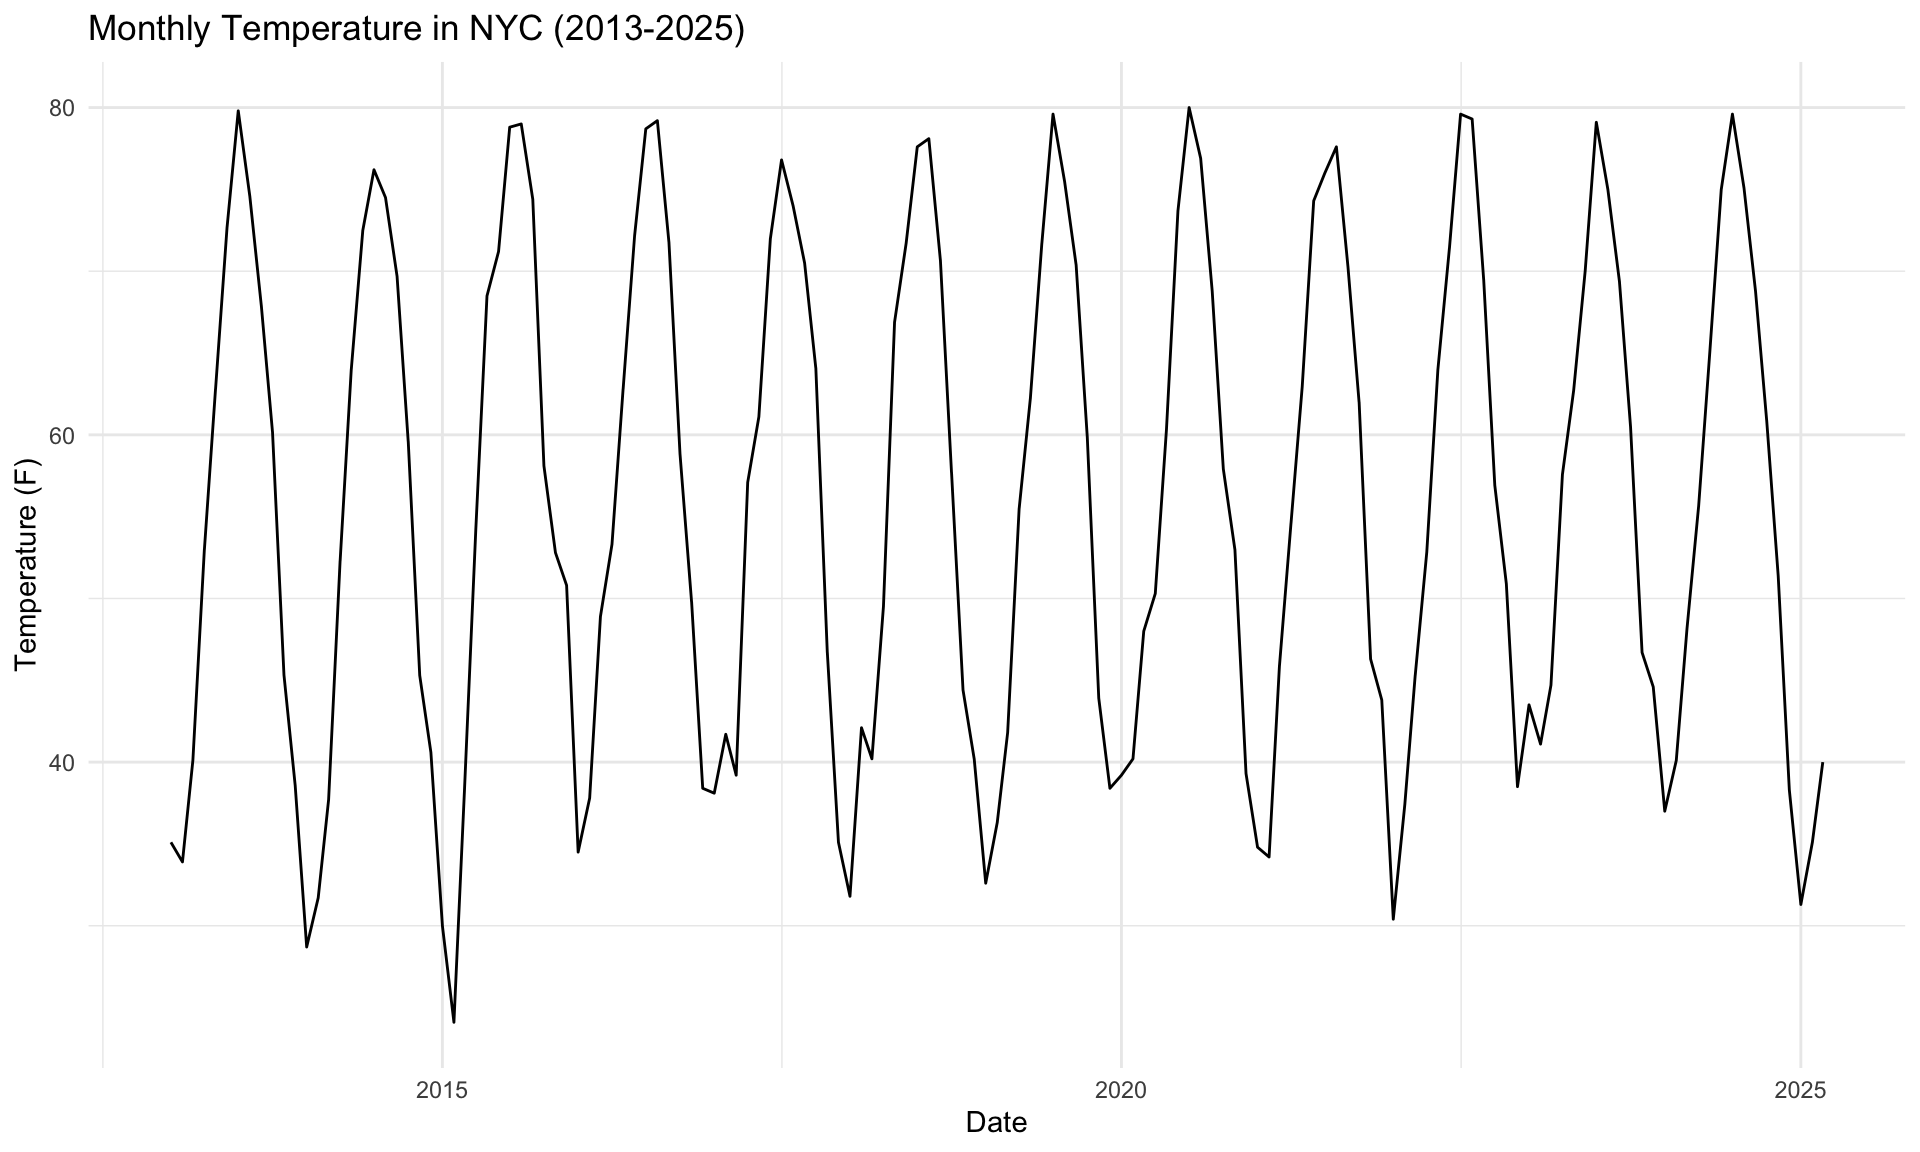
\includegraphics{data_files/figure-pdf/weather-plots-1.pdf}

\begin{Shaded}
\begin{Highlighting}[]
\FunctionTok{ggplot}\NormalTok{(weather\_df, }\FunctionTok{aes}\NormalTok{(}\AttributeTok{x =}\NormalTok{ Date, }\AttributeTok{y =}\NormalTok{ Rainfall)) }\SpecialCharTok{+}
  \FunctionTok{geom\_line}\NormalTok{() }\SpecialCharTok{+}
  \FunctionTok{labs}\NormalTok{(}
    \AttributeTok{title =} \StringTok{"Monthly Rainfall in NYC (2013{-}2025)"}\NormalTok{,}
    \AttributeTok{x =} \StringTok{"Date"}\NormalTok{,}
    \AttributeTok{y =} \StringTok{"Rainfall (inches)"}
\NormalTok{  ) }\SpecialCharTok{+}
  \FunctionTok{theme\_minimal}\NormalTok{()}
\end{Highlighting}
\end{Shaded}

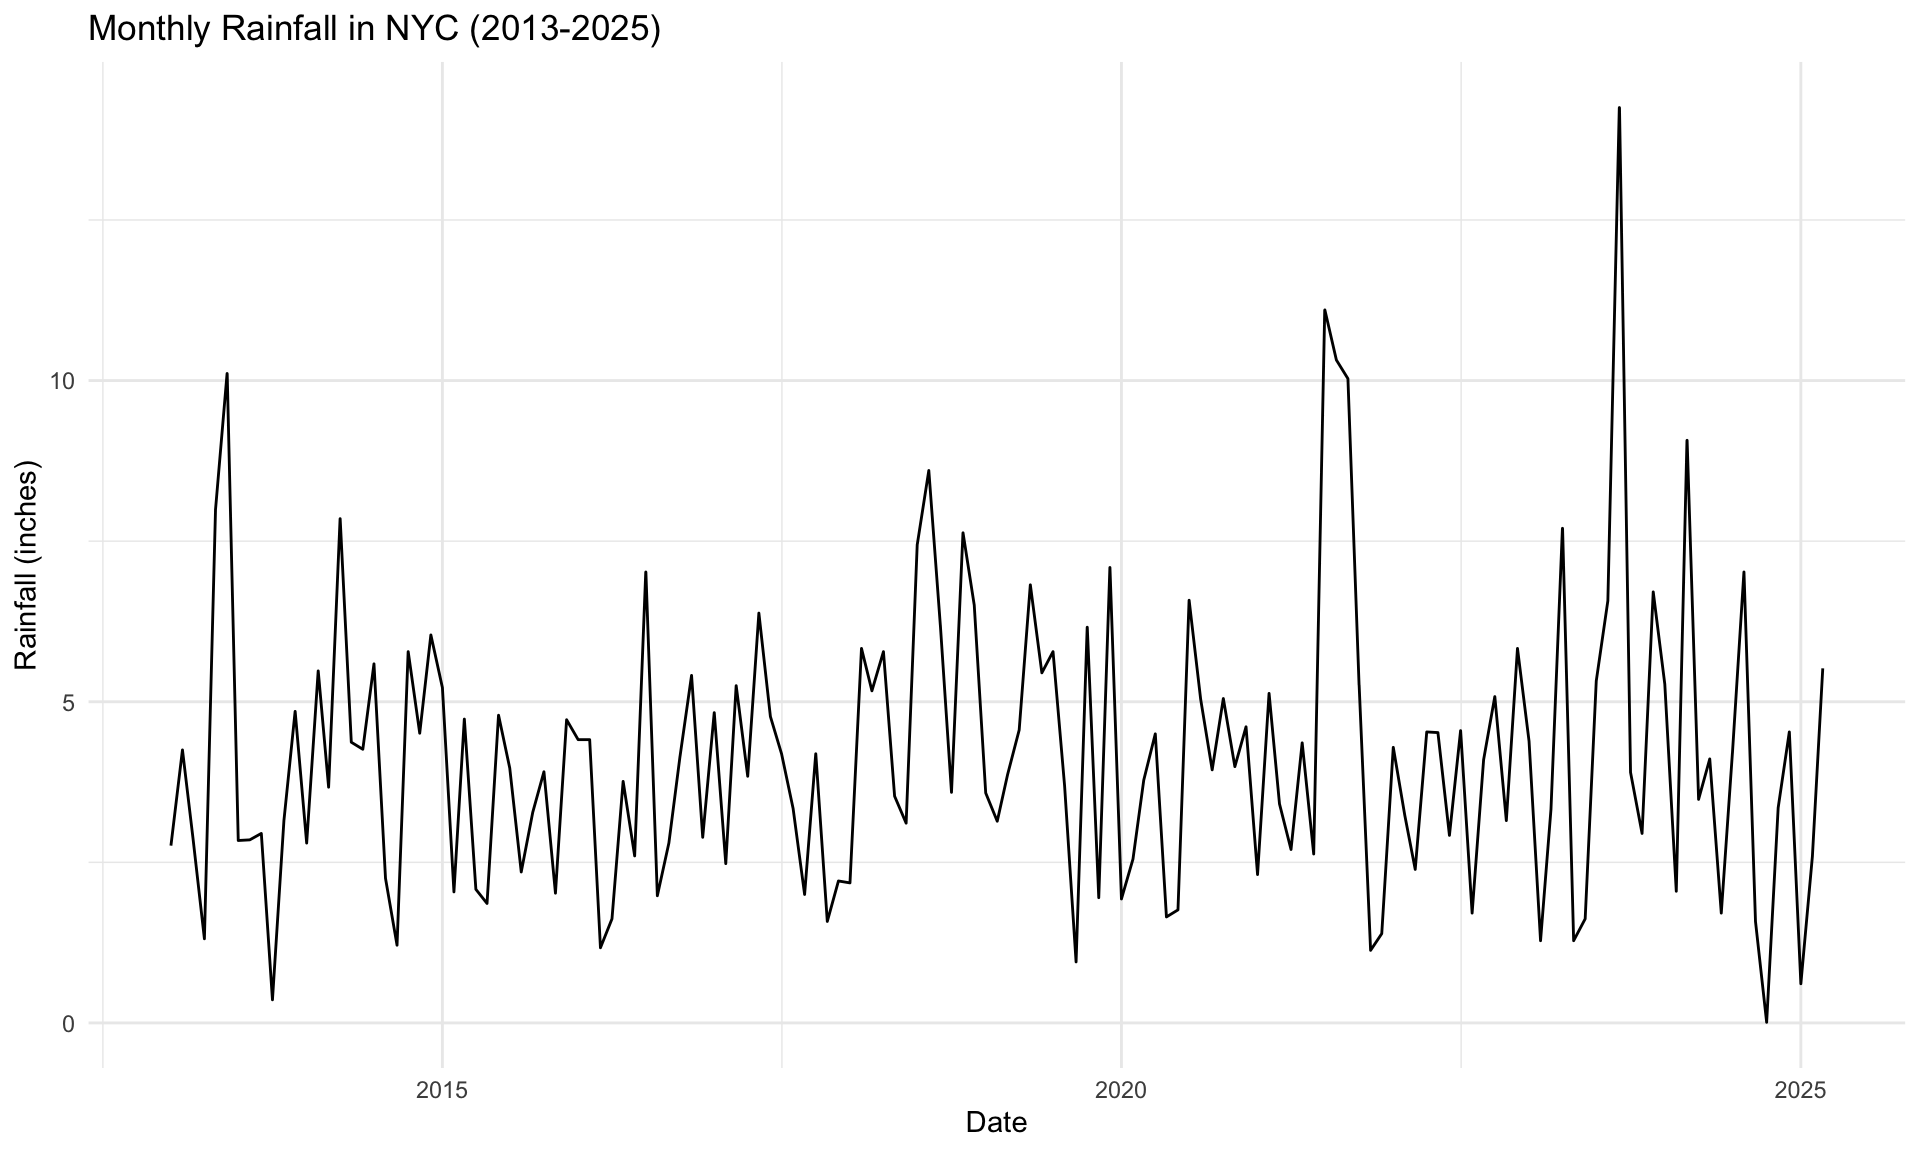
\includegraphics{data_files/figure-pdf/weather-plots-2.pdf}

\begin{Shaded}
\begin{Highlighting}[]
\CommentTok{\# Traffic volume by time of day}
\NormalTok{traffic\_df }\SpecialCharTok{\%\textgreater{}\%}
  \FunctionTok{group\_by}\NormalTok{(TimeOfDay) }\SpecialCharTok{\%\textgreater{}\%}
  \FunctionTok{summarize}\NormalTok{(}\AttributeTok{MeanVolume =} \FunctionTok{mean}\NormalTok{(Vol, }\AttributeTok{na.rm =} \ConstantTok{TRUE}\NormalTok{)) }\SpecialCharTok{\%\textgreater{}\%}
  \FunctionTok{mutate}\NormalTok{(}\AttributeTok{TimeOfDay =} \FunctionTok{factor}\NormalTok{(TimeOfDay, }\AttributeTok{levels =} \FunctionTok{c}\NormalTok{(}\StringTok{"Morning"}\NormalTok{, }\StringTok{"Midday"}\NormalTok{, }\StringTok{"Evening"}\NormalTok{, }\StringTok{"Night"}\NormalTok{))) }\SpecialCharTok{\%\textgreater{}\%}
  \FunctionTok{ggplot}\NormalTok{(}\FunctionTok{aes}\NormalTok{(}\AttributeTok{x =}\NormalTok{ TimeOfDay, }\AttributeTok{y =}\NormalTok{ MeanVolume)) }\SpecialCharTok{+}
  \FunctionTok{geom\_col}\NormalTok{(}\AttributeTok{fill =} \StringTok{"steelblue"}\NormalTok{) }\SpecialCharTok{+}
  \FunctionTok{labs}\NormalTok{(}
    \AttributeTok{title =} \StringTok{"Average Traffic Volume by Time of Day"}\NormalTok{,}
    \AttributeTok{x =} \StringTok{"Time of Day"}\NormalTok{,}
    \AttributeTok{y =} \StringTok{"Average Volume"}
\NormalTok{  ) }\SpecialCharTok{+}
  \FunctionTok{theme\_minimal}\NormalTok{()}

\CommentTok{\# Traffic volume by borough}
\NormalTok{traffic\_df }\SpecialCharTok{\%\textgreater{}\%}
  \FunctionTok{group\_by}\NormalTok{(Boro) }\SpecialCharTok{\%\textgreater{}\%}
  \FunctionTok{summarize}\NormalTok{(}\AttributeTok{MeanVolume =} \FunctionTok{mean}\NormalTok{(Vol, }\AttributeTok{na.rm =} \ConstantTok{TRUE}\NormalTok{)) }\SpecialCharTok{\%\textgreater{}\%}
  \FunctionTok{arrange}\NormalTok{(}\FunctionTok{desc}\NormalTok{(MeanVolume)) }\SpecialCharTok{\%\textgreater{}\%}
  \FunctionTok{ggplot}\NormalTok{(}\FunctionTok{aes}\NormalTok{(}\AttributeTok{x =} \FunctionTok{reorder}\NormalTok{(Boro, MeanVolume), }\AttributeTok{y =}\NormalTok{ MeanVolume)) }\SpecialCharTok{+}
  \FunctionTok{geom\_col}\NormalTok{(}\AttributeTok{fill =} \StringTok{"steelblue"}\NormalTok{) }\SpecialCharTok{+}
  \FunctionTok{labs}\NormalTok{(}
    \AttributeTok{title =} \StringTok{"Average Traffic Volume by Borough"}\NormalTok{,}
    \AttributeTok{x =} \StringTok{"Borough"}\NormalTok{,}
    \AttributeTok{y =} \StringTok{"Average Volume"}
\NormalTok{  ) }\SpecialCharTok{+}
  \FunctionTok{theme\_minimal}\NormalTok{() }\SpecialCharTok{+}
  \FunctionTok{coord\_flip}\NormalTok{()}
\end{Highlighting}
\end{Shaded}

\begin{Shaded}
\begin{Highlighting}[]
\CommentTok{\# Emergency response times by borough}
\FunctionTok{ggplot}\NormalTok{(emergency\_df, }\FunctionTok{aes}\NormalTok{(}\AttributeTok{x =}\NormalTok{ Borough, }\AttributeTok{y =} \StringTok{\textasciigrave{}}\AttributeTok{Response Times}\StringTok{\textasciigrave{}}\NormalTok{)) }\SpecialCharTok{+}
  \FunctionTok{geom\_boxplot}\NormalTok{(}\AttributeTok{fill =} \StringTok{"steelblue"}\NormalTok{, }\AttributeTok{alpha =} \FloatTok{0.7}\NormalTok{) }\SpecialCharTok{+}
  \FunctionTok{labs}\NormalTok{(}
    \AttributeTok{title =} \StringTok{"Emergency Response Times by Borough"}\NormalTok{,}
    \AttributeTok{x =} \StringTok{"Borough"}\NormalTok{,}
    \AttributeTok{y =} \StringTok{"Response Time (seconds)"}
\NormalTok{  ) }\SpecialCharTok{+}
  \FunctionTok{theme\_minimal}\NormalTok{() }\SpecialCharTok{+}
  \FunctionTok{theme}\NormalTok{(}\AttributeTok{axis.text.x =} \FunctionTok{element\_text}\NormalTok{(}\AttributeTok{angle =} \DecValTok{45}\NormalTok{, }\AttributeTok{hjust =} \DecValTok{1}\NormalTok{))}
\end{Highlighting}
\end{Shaded}

\section{Data Integration}\label{data-integration}

\begin{Shaded}
\begin{Highlighting}[]
\CommentTok{\# Function to integrate datasets}
\NormalTok{integrate\_datasets }\OtherTok{\textless{}{-}} \ControlFlowTok{function}\NormalTok{(traffic\_df, weather\_df, emergency\_df) \{}
  \CommentTok{\# Aggregate traffic data to daily level}
\NormalTok{  daily\_traffic }\OtherTok{\textless{}{-}}\NormalTok{ traffic\_df }\SpecialCharTok{\%\textgreater{}\%}
    \FunctionTok{group\_by}\NormalTok{(Year, Month, Day, Boro) }\SpecialCharTok{\%\textgreater{}\%}
    \FunctionTok{summarize}\NormalTok{(}\AttributeTok{Vol =} \FunctionTok{mean}\NormalTok{(Vol, }\AttributeTok{na.rm =} \ConstantTok{TRUE}\NormalTok{), }\AttributeTok{.groups =} \StringTok{"drop"}\NormalTok{) }\SpecialCharTok{\%\textgreater{}\%}
    \FunctionTok{mutate}\NormalTok{(}\AttributeTok{Date =} \FunctionTok{as.Date}\NormalTok{(}\FunctionTok{paste}\NormalTok{(Year, Month, Day, }\AttributeTok{sep =} \StringTok{"{-}"}\NormalTok{)))}
  
  \CommentTok{\# Expand weather data to daily}
\NormalTok{  weather\_expanded }\OtherTok{\textless{}{-}}\NormalTok{ weather\_df }\SpecialCharTok{\%\textgreater{}\%}
    \FunctionTok{select}\NormalTok{(Date, Temperature, Rainfall, TempAnomaly, RainAnomaly, Season) }\SpecialCharTok{\%\textgreater{}\%}
    \FunctionTok{mutate}\NormalTok{(}
      \AttributeTok{month\_start =} \FunctionTok{floor\_date}\NormalTok{(Date, }\StringTok{"month"}\NormalTok{),}
      \AttributeTok{month\_end =} \FunctionTok{ceiling\_date}\NormalTok{(Date, }\StringTok{"month"}\NormalTok{) }\SpecialCharTok{{-}} \FunctionTok{days}\NormalTok{(}\DecValTok{1}\NormalTok{)}
\NormalTok{    )}
  
  \CommentTok{\# Create daily weather records}
\NormalTok{  daily\_weather\_records }\OtherTok{\textless{}{-}} \FunctionTok{list}\NormalTok{()}
  
  \ControlFlowTok{for}\NormalTok{ (i }\ControlFlowTok{in} \DecValTok{1}\SpecialCharTok{:}\FunctionTok{nrow}\NormalTok{(weather\_expanded)) \{}
\NormalTok{    row }\OtherTok{\textless{}{-}}\NormalTok{ weather\_expanded[i, ]}
\NormalTok{    date\_range }\OtherTok{\textless{}{-}} \FunctionTok{seq}\NormalTok{(row}\SpecialCharTok{$}\NormalTok{month\_start, row}\SpecialCharTok{$}\NormalTok{month\_end, }\AttributeTok{by =} \StringTok{"day"}\NormalTok{)}
    
    \ControlFlowTok{for}\NormalTok{ (date }\ControlFlowTok{in}\NormalTok{ date\_range) \{}
\NormalTok{      daily\_record }\OtherTok{\textless{}{-}}\NormalTok{ row}
\NormalTok{      daily\_record}\SpecialCharTok{$}\NormalTok{Date }\OtherTok{\textless{}{-}}\NormalTok{ date}
\NormalTok{      daily\_weather\_records[[}\FunctionTok{length}\NormalTok{(daily\_weather\_records) }\SpecialCharTok{+} \DecValTok{1}\NormalTok{]] }\OtherTok{\textless{}{-}}\NormalTok{ daily\_record}
\NormalTok{    \}}
\NormalTok{  \}}
  
\NormalTok{  daily\_weather }\OtherTok{\textless{}{-}} \FunctionTok{bind\_rows}\NormalTok{(daily\_weather\_records) }\SpecialCharTok{\%\textgreater{}\%}
    \FunctionTok{select}\NormalTok{(}\SpecialCharTok{{-}}\NormalTok{month\_start, }\SpecialCharTok{{-}}\NormalTok{month\_end)}
  
  \CommentTok{\# Merge daily traffic with daily weather}
\NormalTok{  merged\_df }\OtherTok{\textless{}{-}}\NormalTok{ daily\_traffic }\SpecialCharTok{\%\textgreater{}\%}
    \FunctionTok{inner\_join}\NormalTok{(daily\_weather, }\AttributeTok{by =} \StringTok{"Date"}\NormalTok{) }\SpecialCharTok{\%\textgreater{}\%}
    \FunctionTok{mutate}\NormalTok{(}
      \AttributeTok{DayOfWeek =} \FunctionTok{wday}\NormalTok{(Date) }\SpecialCharTok{{-}} \DecValTok{1}\NormalTok{,}
      \AttributeTok{IsWeekend =} \FunctionTok{if\_else}\NormalTok{(DayOfWeek }\SpecialCharTok{\textgreater{}=} \DecValTok{5}\NormalTok{, }\DecValTok{1}\NormalTok{, }\DecValTok{0}\NormalTok{)}
\NormalTok{    )}
  
  \FunctionTok{return}\NormalTok{(merged\_df)}
\NormalTok{\}}

\CommentTok{\# Integrate datasets}
\NormalTok{integrated\_data }\OtherTok{\textless{}{-}} \FunctionTok{integrate\_datasets}\NormalTok{(traffic\_df, weather\_df, emergency\_df)}

\CommentTok{\# Save processed data}
\FunctionTok{write\_csv}\NormalTok{(weather\_df, }\FunctionTok{here}\NormalTok{(}\StringTok{"data"}\NormalTok{, }\StringTok{"processed\_weather\_data.csv"}\NormalTok{))}
\FunctionTok{write\_csv}\NormalTok{(traffic\_df, }\FunctionTok{here}\NormalTok{(}\StringTok{"data"}\NormalTok{, }\StringTok{"processed\_traffic\_data.csv"}\NormalTok{))}
\FunctionTok{write\_csv}\NormalTok{(emergency\_df, }\FunctionTok{here}\NormalTok{(}\StringTok{"data"}\NormalTok{, }\StringTok{"processed\_emergency\_data.csv"}\NormalTok{))}
\FunctionTok{write\_csv}\NormalTok{(integrated\_data, }\FunctionTok{here}\NormalTok{(}\StringTok{"data"}\NormalTok{, }\StringTok{"integrated\_data.csv"}\NormalTok{))}

\CommentTok{\# Display the structure of the integrated dataset}
\FunctionTok{glimpse}\NormalTok{(integrated\_data)}
\end{Highlighting}
\end{Shaded}

\section{Feature Engineering}\label{feature-engineering}

\begin{Shaded}
\begin{Highlighting}[]
\CommentTok{\# Function to engineer features}
\NormalTok{engineer\_features }\OtherTok{\textless{}{-}} \ControlFlowTok{function}\NormalTok{(df) \{}
  \CommentTok{\# One{-}hot encode categorical variables}
\NormalTok{  df }\OtherTok{\textless{}{-}}\NormalTok{ df }\SpecialCharTok{\%\textgreater{}\%}
    \FunctionTok{mutate}\NormalTok{(}
      \AttributeTok{Season\_Spring =} \FunctionTok{if\_else}\NormalTok{(Season }\SpecialCharTok{==} \StringTok{"Spring"}\NormalTok{, }\DecValTok{1}\NormalTok{, }\DecValTok{0}\NormalTok{),}
      \AttributeTok{Season\_Summer =} \FunctionTok{if\_else}\NormalTok{(Season }\SpecialCharTok{==} \StringTok{"Summer"}\NormalTok{, }\DecValTok{1}\NormalTok{, }\DecValTok{0}\NormalTok{),}
      \AttributeTok{Season\_Fall =} \FunctionTok{if\_else}\NormalTok{(Season }\SpecialCharTok{==} \StringTok{"Fall"}\NormalTok{, }\DecValTok{1}\NormalTok{, }\DecValTok{0}\NormalTok{),}
      \AttributeTok{Season\_Winter =} \FunctionTok{if\_else}\NormalTok{(Season }\SpecialCharTok{==} \StringTok{"Winter"}\NormalTok{, }\DecValTok{1}\NormalTok{, }\DecValTok{0}\NormalTok{)}
\NormalTok{    )}
  
  \CommentTok{\# Create borough dummy variables}
\NormalTok{  boroughs }\OtherTok{\textless{}{-}} \FunctionTok{unique}\NormalTok{(df}\SpecialCharTok{$}\NormalTok{Boro)}
  \ControlFlowTok{for}\NormalTok{ (borough }\ControlFlowTok{in}\NormalTok{ boroughs) \{}
\NormalTok{    col\_name }\OtherTok{\textless{}{-}} \FunctionTok{paste0}\NormalTok{(}\StringTok{"Boro\_"}\NormalTok{, borough)}
\NormalTok{    df[[col\_name]] }\OtherTok{\textless{}{-}} \FunctionTok{if\_else}\NormalTok{(df}\SpecialCharTok{$}\NormalTok{Boro }\SpecialCharTok{==}\NormalTok{ borough, }\DecValTok{1}\NormalTok{, }\DecValTok{0}\NormalTok{)}
\NormalTok{  \}}
  
  \CommentTok{\# Add lagged features (previous day\textquotesingle{}s traffic volume)}
  \ControlFlowTok{for}\NormalTok{ (borough }\ControlFlowTok{in}\NormalTok{ boroughs) \{}
\NormalTok{    col\_name }\OtherTok{\textless{}{-}} \FunctionTok{paste0}\NormalTok{(}\StringTok{"Boro\_"}\NormalTok{, borough)}
\NormalTok{    lag\_col\_name }\OtherTok{\textless{}{-}} \FunctionTok{paste0}\NormalTok{(borough, }\StringTok{"\_prev\_day\_vol"}\NormalTok{)}
    
    \CommentTok{\# Filter for this borough and sort by date}
\NormalTok{    boro\_data }\OtherTok{\textless{}{-}}\NormalTok{ df }\SpecialCharTok{\%\textgreater{}\%}
      \FunctionTok{filter}\NormalTok{(}\SpecialCharTok{!!}\FunctionTok{sym}\NormalTok{(col\_name) }\SpecialCharTok{==} \DecValTok{1}\NormalTok{) }\SpecialCharTok{\%\textgreater{}\%}
      \FunctionTok{arrange}\NormalTok{(Date)}
    
    \CommentTok{\# Create lagged volume}
\NormalTok{    boro\_data }\OtherTok{\textless{}{-}}\NormalTok{ boro\_data }\SpecialCharTok{\%\textgreater{}\%}
      \FunctionTok{mutate}\NormalTok{(}\SpecialCharTok{!!}\AttributeTok{lag\_col\_name :=} \FunctionTok{lag}\NormalTok{(Vol))}
    
    \CommentTok{\# Update the original dataframe}
\NormalTok{    df }\OtherTok{\textless{}{-}}\NormalTok{ df }\SpecialCharTok{\%\textgreater{}\%}
      \FunctionTok{left\_join}\NormalTok{(}
\NormalTok{        boro\_data }\SpecialCharTok{\%\textgreater{}\%} \FunctionTok{select}\NormalTok{(Date, Boro, }\SpecialCharTok{!!}\NormalTok{lag\_col\_name),}
        \AttributeTok{by =} \FunctionTok{c}\NormalTok{(}\StringTok{"Date"}\NormalTok{, }\StringTok{"Boro"}\NormalTok{)}
\NormalTok{      )}
\NormalTok{  \}}
  
  \CommentTok{\# Fill NA values from lagged features with mean values}
  \ControlFlowTok{for}\NormalTok{ (col }\ControlFlowTok{in} \FunctionTok{names}\NormalTok{(df)) \{}
    \ControlFlowTok{if}\NormalTok{ (}\FunctionTok{any}\NormalTok{(}\FunctionTok{is.na}\NormalTok{(df[[col]]))) \{}
\NormalTok{      col\_mean }\OtherTok{\textless{}{-}} \FunctionTok{mean}\NormalTok{(df[[col]], }\AttributeTok{na.rm =} \ConstantTok{TRUE}\NormalTok{)}
\NormalTok{      df[[col]] }\OtherTok{\textless{}{-}} \FunctionTok{if\_else}\NormalTok{(}\FunctionTok{is.na}\NormalTok{(df[[col]]), col\_mean, df[[col]])}
\NormalTok{    \}}
\NormalTok{  \}}
  
  \FunctionTok{return}\NormalTok{(df)}
\NormalTok{\}}

\CommentTok{\# Engineer features}
\NormalTok{engineered\_data }\OtherTok{\textless{}{-}} \FunctionTok{engineer\_features}\NormalTok{(integrated\_data)}

\CommentTok{\# Save engineered data}
\FunctionTok{write\_csv}\NormalTok{(engineered\_data, }\FunctionTok{here}\NormalTok{(}\StringTok{"data"}\NormalTok{, }\StringTok{"engineered\_data.csv"}\NormalTok{))}

\CommentTok{\# Summary of engineered features}
\FunctionTok{summary}\NormalTok{(engineered\_data)}
\end{Highlighting}
\end{Shaded}

\section{Summary}\label{summary}

\begin{enumerate}
\def\labelenumi{\arabic{enumi}.}
\tightlist
\item
  \textbf{Loaded and cleaned} three distinct datasets: traffic volumes,
  weather patterns, and emergency response times
\item
  \textbf{Created time-based features} including time of day, day of
  week, and seasonal indicators
\item
  \textbf{Performed exploratory visualizations} to understand traffic
  patterns by time and location
\item
  \textbf{Integrated the datasets} to create a comprehensive view of NYC
  traffic patterns
\item
  \textbf{Engineered additional features} to improve the model's
  predictive capabilities
\end{enumerate}

The prepared data will be called in the next chapter to develop the
models and analysis.

\bookmarksetup{startatroot}

\chapter{Model Development and
Interpretation}\label{model-development-and-interpretation}

This chapter is on the predictive models to look into the factors
driving NYC traffic congestion.

\section{Setup}\label{setup}

Load the necessary libraries and preprocessed data:

\section{Loading Preprocessed Data}\label{loading-preprocessed-data}

Use the raw traffic CSV for modeling:

\begin{Shaded}
\begin{Highlighting}[]
\CommentTok{\# Load raw traffic data for modeling}
\NormalTok{model\_data }\OtherTok{\textless{}{-}} \FunctionTok{read\_csv}\NormalTok{(}\FunctionTok{here}\NormalTok{(}\StringTok{"data"}\NormalTok{, }\StringTok{"Automated\_Traffic\_Volume\_Counts\_20250505.csv"}\NormalTok{))}
\end{Highlighting}
\end{Shaded}

\begin{verbatim}
Rows: 1712605 Columns: 14
-- Column specification --------------------------------------------------------
Delimiter: ","
chr (6): Boro, WktGeom, street, fromSt, toSt, Direction
dbl (8): RequestID, Yr, M, D, HH, MM, Vol, SegmentID

i Use `spec()` to retrieve the full column specification for this data.
i Specify the column types or set `show_col_types = FALSE` to quiet this message.
\end{verbatim}

\begin{Shaded}
\begin{Highlighting}[]
\CommentTok{\# Display structure}
\FunctionTok{glimpse}\NormalTok{(model\_data)}
\end{Highlighting}
\end{Shaded}

\begin{verbatim}
Rows: 1,712,605
Columns: 14
$ RequestID <dbl> 32970, 32970, 11342, 32970, 32970, 32970, 32970, 32970, 3297~
$ Boro      <chr> "Queens", "Queens", "Brooklyn", "Queens", "Queens", "Queens"~
$ Yr        <dbl> 2021, 2021, 2012, 2021, 2021, 2021, 2021, 2021, 2021, 2021, ~
$ M         <dbl> 4, 4, 12, 4, 4, 4, 4, 4, 4, 4, 4, 4, 4, 4, 4, 4, 4, 4, 4, 4,~
$ D         <dbl> 30, 30, 18, 30, 30, 30, 30, 30, 30, 30, 30, 30, 30, 30, 30, ~
$ HH        <dbl> 2, 2, 8, 2, 2, 3, 3, 3, 3, 4, 4, 4, 4, 5, 5, 5, 5, 6, 6, 6, ~
$ MM        <dbl> 0, 15, 15, 30, 45, 0, 15, 30, 45, 0, 15, 30, 45, 0, 15, 30, ~
$ Vol       <dbl> 0, 1, 33, 0, 0, 1, 0, 0, 1, 0, 0, 0, 1, 2, 4, 16, 5, 11, 9, ~
$ SegmentID <dbl> 149701, 149701, 20063, 149701, 149701, 149701, 149701, 14970~
$ WktGeom   <chr> "POINT (997407.0998491726 208620.92612708386)", "POINT (9974~
$ street    <chr> "PULASKI BRIDGE", "PULASKI BRIDGE", "61 ST", "PULASKI BRIDGE~
$ fromSt    <chr> "Newtown Creek Shoreline", "Newtown Creek Shoreline", "15 AV~
$ toSt      <chr> "Dead end", "Dead end", "16 AV", "Dead end", "Dead end", "De~
$ Direction <chr> "NB", "NB", "WB", "NB", "NB", "NB", "NB", "NB", "NB", "NB", ~
\end{verbatim}

\section{Data Preparation for
Modeling}\label{data-preparation-for-modeling}

Split the data into training and testing sets, and prepare the feature
set:

\begin{Shaded}
\begin{Highlighting}[]
\CommentTok{\# Function to prepare data for modeling}
\NormalTok{prepare\_data\_for\_modeling }\OtherTok{\textless{}{-}} \ControlFlowTok{function}\NormalTok{(df, }\AttributeTok{target\_col =} \StringTok{"Vol"}\NormalTok{, }\AttributeTok{test\_size =} \FloatTok{0.2}\NormalTok{) \{}
  \CommentTok{\# Remove raw identifier columns not used in modeling}
\NormalTok{  features }\OtherTok{\textless{}{-}}\NormalTok{ df }\SpecialCharTok{\%\textgreater{}\%}
    \FunctionTok{select}\NormalTok{(}\SpecialCharTok{{-}}\FunctionTok{c}\NormalTok{(Yr, M, D, HH, MM, Boro, WktGeom, street, fromSt, toSt))}
  
  \CommentTok{\# Create the temporal split}
\NormalTok{  train\_size }\OtherTok{\textless{}{-}} \FunctionTok{floor}\NormalTok{((}\DecValTok{1} \SpecialCharTok{{-}}\NormalTok{ test\_size) }\SpecialCharTok{*} \FunctionTok{nrow}\NormalTok{(features))}
\NormalTok{  train\_indices }\OtherTok{\textless{}{-}} \DecValTok{1}\SpecialCharTok{:}\NormalTok{train\_size}
  
  \CommentTok{\# Split data}
\NormalTok{  X\_train }\OtherTok{\textless{}{-}}\NormalTok{ features[train\_indices, ] }\SpecialCharTok{\%\textgreater{}\%} \FunctionTok{select}\NormalTok{(}\SpecialCharTok{{-}}\FunctionTok{all\_of}\NormalTok{(target\_col))}
\NormalTok{  X\_test }\OtherTok{\textless{}{-}}\NormalTok{ features[}\SpecialCharTok{{-}}\NormalTok{train\_indices, ] }\SpecialCharTok{\%\textgreater{}\%} \FunctionTok{select}\NormalTok{(}\SpecialCharTok{{-}}\FunctionTok{all\_of}\NormalTok{(target\_col))}
\NormalTok{  y\_train }\OtherTok{\textless{}{-}}\NormalTok{ features[train\_indices, ] }\SpecialCharTok{\%\textgreater{}\%} \FunctionTok{pull}\NormalTok{(target\_col)}
\NormalTok{  y\_test }\OtherTok{\textless{}{-}}\NormalTok{ features[}\SpecialCharTok{{-}}\NormalTok{train\_indices, ] }\SpecialCharTok{\%\textgreater{}\%} \FunctionTok{pull}\NormalTok{(target\_col)}
  
  \CommentTok{\# Create recipe for preprocessing}
\NormalTok{  model\_recipe }\OtherTok{\textless{}{-}} \FunctionTok{recipe}\NormalTok{(}\SpecialCharTok{\textasciitilde{}}\NormalTok{ ., }\AttributeTok{data =}\NormalTok{ X\_train) }\SpecialCharTok{\%\textgreater{}\%}
    \FunctionTok{step\_normalize}\NormalTok{(}\FunctionTok{all\_numeric\_predictors}\NormalTok{())}
  
  \CommentTok{\# Prepare the recipe}
\NormalTok{  model\_prep }\OtherTok{\textless{}{-}} \FunctionTok{prep}\NormalTok{(model\_recipe)}
  
  \CommentTok{\# Apply the recipe}
\NormalTok{  X\_train\_processed }\OtherTok{\textless{}{-}} \FunctionTok{bake}\NormalTok{(model\_prep, }\AttributeTok{new\_data =}\NormalTok{ X\_train)}
\NormalTok{  X\_test\_processed }\OtherTok{\textless{}{-}} \FunctionTok{bake}\NormalTok{(model\_prep, }\AttributeTok{new\_data =}\NormalTok{ X\_test)}
  
  \FunctionTok{return}\NormalTok{(}\FunctionTok{list}\NormalTok{(}
    \AttributeTok{X\_train =}\NormalTok{ X\_train,}
    \AttributeTok{X\_test =}\NormalTok{ X\_test,}
    \AttributeTok{y\_train =}\NormalTok{ y\_train,}
    \AttributeTok{y\_test =}\NormalTok{ y\_test,}
    \AttributeTok{X\_train\_processed =}\NormalTok{ X\_train\_processed,}
    \AttributeTok{X\_test\_processed =}\NormalTok{ X\_test\_processed,}
    \AttributeTok{recipe =}\NormalTok{ model\_recipe}
\NormalTok{  ))}
\NormalTok{\}}

\CommentTok{\# Prepare data}
\NormalTok{model\_data\_split }\OtherTok{\textless{}{-}} \FunctionTok{prepare\_data\_for\_modeling}\NormalTok{(model\_data)}

\CommentTok{\# Check dimensions}
\FunctionTok{cat}\NormalTok{(}\StringTok{"Training features:"}\NormalTok{, }\FunctionTok{dim}\NormalTok{(model\_data\_split}\SpecialCharTok{$}\NormalTok{X\_train), }\StringTok{"}\SpecialCharTok{\textbackslash{}n}\StringTok{"}\NormalTok{)}
\end{Highlighting}
\end{Shaded}

\begin{verbatim}
Training features: 1370084 3 
\end{verbatim}

\begin{Shaded}
\begin{Highlighting}[]
\FunctionTok{cat}\NormalTok{(}\StringTok{"Testing features:"}\NormalTok{, }\FunctionTok{dim}\NormalTok{(model\_data\_split}\SpecialCharTok{$}\NormalTok{X\_test), }\StringTok{"}\SpecialCharTok{\textbackslash{}n}\StringTok{"}\NormalTok{)}
\end{Highlighting}
\end{Shaded}

\begin{verbatim}
Testing features: 342521 3 
\end{verbatim}

\section{Model Development}\label{model-development}

Train multiple models to predict traffic volume:

\begin{Shaded}
\begin{Highlighting}[]
\CommentTok{\# Function to train different models}
\NormalTok{train\_models }\OtherTok{\textless{}{-}} \ControlFlowTok{function}\NormalTok{(X\_train, X\_test, y\_train, y\_test, X\_train\_processed, X\_test\_processed) \{}
\NormalTok{  models }\OtherTok{\textless{}{-}} \FunctionTok{list}\NormalTok{()}
\NormalTok{  results }\OtherTok{\textless{}{-}} \FunctionTok{list}\NormalTok{()}
  
  \CommentTok{\# 1. Linear Regression (baseline)}
  \FunctionTok{cat}\NormalTok{(}\StringTok{"Training Linear Regression...}\SpecialCharTok{\textbackslash{}n}\StringTok{"}\NormalTok{)}
\NormalTok{  lm\_model }\OtherTok{\textless{}{-}} \FunctionTok{linear\_reg}\NormalTok{() }\SpecialCharTok{\%\textgreater{}\%}
    \FunctionTok{set\_engine}\NormalTok{(}\StringTok{"lm"}\NormalTok{) }\SpecialCharTok{\%\textgreater{}\%}
    \FunctionTok{fit}\NormalTok{(}
\NormalTok{      target }\SpecialCharTok{\textasciitilde{}}\NormalTok{ .,}
      \AttributeTok{data =} \FunctionTok{bind\_cols}\NormalTok{(X\_train\_processed, }\AttributeTok{target =}\NormalTok{ y\_train)}
\NormalTok{    )}
  
\NormalTok{  lm\_preds }\OtherTok{\textless{}{-}} \FunctionTok{predict}\NormalTok{(lm\_model, }\AttributeTok{new\_data =}\NormalTok{ X\_test\_processed)}\SpecialCharTok{$}\NormalTok{.pred}
\NormalTok{  models[[}\StringTok{"Linear"}\NormalTok{]] }\OtherTok{\textless{}{-}}\NormalTok{ lm\_model}
  
  \CommentTok{\# Calculate metrics}
\NormalTok{  lm\_rmse }\OtherTok{\textless{}{-}} \FunctionTok{sqrt}\NormalTok{(}\FunctionTok{mean}\NormalTok{((lm\_preds }\SpecialCharTok{{-}}\NormalTok{ y\_test)}\SpecialCharTok{\^{}}\DecValTok{2}\NormalTok{))}
\NormalTok{  lm\_r2 }\OtherTok{\textless{}{-}} \FunctionTok{cor}\NormalTok{(lm\_preds, y\_test)}\SpecialCharTok{\^{}}\DecValTok{2}
  
\NormalTok{  results[[}\StringTok{"Linear"}\NormalTok{]] }\OtherTok{\textless{}{-}} \FunctionTok{list}\NormalTok{(}
    \AttributeTok{rmse =}\NormalTok{ lm\_rmse,}
    \AttributeTok{r2 =}\NormalTok{ lm\_r2,}
    \AttributeTok{feature\_importance =}\NormalTok{ lm\_model}\SpecialCharTok{$}\NormalTok{fit}\SpecialCharTok{$}\NormalTok{coefficients[}\SpecialCharTok{{-}}\DecValTok{1}\NormalTok{] }\CommentTok{\# Exclude intercept}
\NormalTok{  )}
  
  \CommentTok{\# 2. Random Forest}
  \FunctionTok{cat}\NormalTok{(}\StringTok{"Training Random Forest...}\SpecialCharTok{\textbackslash{}n}\StringTok{"}\NormalTok{)}
\NormalTok{  rf\_model }\OtherTok{\textless{}{-}} \FunctionTok{rand\_forest}\NormalTok{(}\AttributeTok{trees =} \DecValTok{100}\NormalTok{) }\SpecialCharTok{\%\textgreater{}\%}
    \FunctionTok{set\_engine}\NormalTok{(}\StringTok{"ranger"}\NormalTok{, }\AttributeTok{importance =} \StringTok{"impurity"}\NormalTok{) }\SpecialCharTok{\%\textgreater{}\%}
    \FunctionTok{set\_mode}\NormalTok{(}\StringTok{"regression"}\NormalTok{) }\SpecialCharTok{\%\textgreater{}\%}
    \FunctionTok{fit}\NormalTok{(}
\NormalTok{      target }\SpecialCharTok{\textasciitilde{}}\NormalTok{ .,}
      \AttributeTok{data =} \FunctionTok{bind\_cols}\NormalTok{(X\_train, }\AttributeTok{target =}\NormalTok{ y\_train)}
\NormalTok{    )}
  
\NormalTok{  rf\_preds }\OtherTok{\textless{}{-}} \FunctionTok{predict}\NormalTok{(rf\_model, }\AttributeTok{new\_data =}\NormalTok{ X\_test)}\SpecialCharTok{$}\NormalTok{.pred}
\NormalTok{  models[[}\StringTok{"RF"}\NormalTok{]] }\OtherTok{\textless{}{-}}\NormalTok{ rf\_model}
  
  \CommentTok{\# Calculate metrics and feature importance}
\NormalTok{  rf\_rmse }\OtherTok{\textless{}{-}} \FunctionTok{sqrt}\NormalTok{(}\FunctionTok{mean}\NormalTok{((rf\_preds }\SpecialCharTok{{-}}\NormalTok{ y\_test)}\SpecialCharTok{\^{}}\DecValTok{2}\NormalTok{))}
\NormalTok{  rf\_r2 }\OtherTok{\textless{}{-}} \FunctionTok{cor}\NormalTok{(rf\_preds, y\_test)}\SpecialCharTok{\^{}}\DecValTok{2}
\NormalTok{  rf\_importance }\OtherTok{\textless{}{-}}\NormalTok{ ranger}\SpecialCharTok{::}\FunctionTok{importance}\NormalTok{(rf\_model}\SpecialCharTok{$}\NormalTok{fit)}
  
\NormalTok{  results[[}\StringTok{"RF"}\NormalTok{]] }\OtherTok{\textless{}{-}} \FunctionTok{list}\NormalTok{(}
    \AttributeTok{rmse =}\NormalTok{ rf\_rmse,}
    \AttributeTok{r2 =}\NormalTok{ rf\_r2,}
    \AttributeTok{feature\_importance =}\NormalTok{ rf\_importance}
\NormalTok{  )}
  
  \CommentTok{\# 3. XGBoost}
  \FunctionTok{cat}\NormalTok{(}\StringTok{"Training XGBoost...}\SpecialCharTok{\textbackslash{}n}\StringTok{"}\NormalTok{)}
  \CommentTok{\# Convert character columns to numeric codes for XGBoost}
\NormalTok{  X\_train\_matrix }\OtherTok{\textless{}{-}}\NormalTok{ X\_train }\SpecialCharTok{\%\textgreater{}\%}
    \FunctionTok{mutate}\NormalTok{(}\FunctionTok{across}\NormalTok{(}\FunctionTok{where}\NormalTok{(is.character), }\SpecialCharTok{\textasciitilde{}} \FunctionTok{as.numeric}\NormalTok{(}\FunctionTok{as.factor}\NormalTok{(.)))) }\SpecialCharTok{\%\textgreater{}\%}
    \FunctionTok{as.matrix}\NormalTok{()}
\NormalTok{  X\_test\_matrix }\OtherTok{\textless{}{-}}\NormalTok{ X\_test }\SpecialCharTok{\%\textgreater{}\%}
    \FunctionTok{mutate}\NormalTok{(}\FunctionTok{across}\NormalTok{(}\FunctionTok{where}\NormalTok{(is.character), }\SpecialCharTok{\textasciitilde{}} \FunctionTok{as.numeric}\NormalTok{(}\FunctionTok{as.factor}\NormalTok{(.)))) }\SpecialCharTok{\%\textgreater{}\%}
    \FunctionTok{as.matrix}\NormalTok{()}
\NormalTok{  xgb\_train }\OtherTok{\textless{}{-}} \FunctionTok{xgb.DMatrix}\NormalTok{(}\AttributeTok{data =}\NormalTok{ X\_train\_matrix, }\AttributeTok{label =}\NormalTok{ y\_train)}
\NormalTok{  xgb\_test }\OtherTok{\textless{}{-}} \FunctionTok{xgb.DMatrix}\NormalTok{(}\AttributeTok{data =}\NormalTok{ X\_test\_matrix, }\AttributeTok{label =}\NormalTok{ y\_test)}
  
\NormalTok{  xgb\_params }\OtherTok{\textless{}{-}} \FunctionTok{list}\NormalTok{(}
    \AttributeTok{objective =} \StringTok{"reg:squarederror"}\NormalTok{,}
    \AttributeTok{eta =} \FloatTok{0.1}\NormalTok{,}
    \AttributeTok{max\_depth =} \DecValTok{6}\NormalTok{,}
    \AttributeTok{nrounds =} \DecValTok{100}
\NormalTok{  )}
  
\NormalTok{  xgb\_model }\OtherTok{\textless{}{-}} \FunctionTok{xgb.train}\NormalTok{(}
    \AttributeTok{params =}\NormalTok{ xgb\_params,}
    \AttributeTok{data =}\NormalTok{ xgb\_train,}
    \AttributeTok{nrounds =} \DecValTok{100}\NormalTok{,}
    \AttributeTok{watchlist =} \FunctionTok{list}\NormalTok{(}\AttributeTok{train =}\NormalTok{ xgb\_train, }\AttributeTok{test =}\NormalTok{ xgb\_test),}
    \AttributeTok{verbose =} \DecValTok{0}
\NormalTok{  )}
  
\NormalTok{  xgb\_preds }\OtherTok{\textless{}{-}} \FunctionTok{predict}\NormalTok{(xgb\_model, xgb\_test)}
\NormalTok{  models[[}\StringTok{"XGB"}\NormalTok{]] }\OtherTok{\textless{}{-}}\NormalTok{ xgb\_model}
  
  \CommentTok{\# Calculate metrics and feature importance}
\NormalTok{  xgb\_rmse }\OtherTok{\textless{}{-}} \FunctionTok{sqrt}\NormalTok{(}\FunctionTok{mean}\NormalTok{((xgb\_preds }\SpecialCharTok{{-}}\NormalTok{ y\_test)}\SpecialCharTok{\^{}}\DecValTok{2}\NormalTok{))}
\NormalTok{  xgb\_r2 }\OtherTok{\textless{}{-}} \FunctionTok{cor}\NormalTok{(xgb\_preds, y\_test)}\SpecialCharTok{\^{}}\DecValTok{2}
\NormalTok{  xgb\_importance }\OtherTok{\textless{}{-}} \FunctionTok{xgb.importance}\NormalTok{(}\AttributeTok{model =}\NormalTok{ xgb\_model)}
  
\NormalTok{  results[[}\StringTok{"XGB"}\NormalTok{]] }\OtherTok{\textless{}{-}} \FunctionTok{list}\NormalTok{(}
    \AttributeTok{rmse =}\NormalTok{ xgb\_rmse,}
    \AttributeTok{r2 =}\NormalTok{ xgb\_r2,}
    \AttributeTok{feature\_importance =} \FunctionTok{setNames}\NormalTok{(xgb\_importance}\SpecialCharTok{$}\NormalTok{Gain, xgb\_importance}\SpecialCharTok{$}\NormalTok{Feature)}
\NormalTok{  )}
  
  \FunctionTok{return}\NormalTok{(}\FunctionTok{list}\NormalTok{(}\AttributeTok{models =}\NormalTok{ models, }\AttributeTok{results =}\NormalTok{ results))}
\NormalTok{\}}

\CommentTok{\# Train models}
\NormalTok{model\_results }\OtherTok{\textless{}{-}} \FunctionTok{train\_models}\NormalTok{(}
\NormalTok{  model\_data\_split}\SpecialCharTok{$}\NormalTok{X\_train,}
\NormalTok{  model\_data\_split}\SpecialCharTok{$}\NormalTok{X\_test,}
\NormalTok{  model\_data\_split}\SpecialCharTok{$}\NormalTok{y\_train,}
\NormalTok{  model\_data\_split}\SpecialCharTok{$}\NormalTok{y\_test,}
\NormalTok{  model\_data\_split}\SpecialCharTok{$}\NormalTok{X\_train\_processed,}
\NormalTok{  model\_data\_split}\SpecialCharTok{$}\NormalTok{X\_test\_processed}
\NormalTok{)}
\end{Highlighting}
\end{Shaded}

\begin{verbatim}
Training Linear Regression...
Training Random Forest...
Training XGBoost...
[18:10:10] WARNING: src/learner.cc:767: 
Parameters: { "nrounds" } are not used.
\end{verbatim}

\begin{Shaded}
\begin{Highlighting}[]
\NormalTok{models }\OtherTok{\textless{}{-}}\NormalTok{ model\_results}\SpecialCharTok{$}\NormalTok{models}
\NormalTok{results }\OtherTok{\textless{}{-}}\NormalTok{ model\_results}\SpecialCharTok{$}\NormalTok{results}

\CommentTok{\# Compare model performance}
\NormalTok{performance\_df }\OtherTok{\textless{}{-}} \FunctionTok{tibble}\NormalTok{(}
  \AttributeTok{Model =} \FunctionTok{names}\NormalTok{(results),}
  \AttributeTok{RMSE =} \FunctionTok{sapply}\NormalTok{(results, }\ControlFlowTok{function}\NormalTok{(x) x}\SpecialCharTok{$}\NormalTok{rmse),}
  \AttributeTok{R2 =} \FunctionTok{sapply}\NormalTok{(results, }\ControlFlowTok{function}\NormalTok{(x) x}\SpecialCharTok{$}\NormalTok{r2)}
\NormalTok{)}

\NormalTok{performance\_df}
\end{Highlighting}
\end{Shaded}

\begin{verbatim}
# A tibble: 3 x 3
  Model   RMSE      R2
  <chr>  <dbl>   <dbl>
1 Linear  123. 0.00423
2 RF      106. 0.240  
3 XGB     102. 0.306  
\end{verbatim}

\section{Model Performance
Visualization}\label{model-performance-visualization}

Visualize the performance of the models:

\begin{Shaded}
\begin{Highlighting}[]
\CommentTok{\# Plot R² comparison}
\FunctionTok{ggplot}\NormalTok{(performance\_df, }\FunctionTok{aes}\NormalTok{(}\AttributeTok{x =}\NormalTok{ Model, }\AttributeTok{y =}\NormalTok{ R2, }\AttributeTok{fill =}\NormalTok{ Model)) }\SpecialCharTok{+}
  \FunctionTok{geom\_col}\NormalTok{() }\SpecialCharTok{+}
  \FunctionTok{scale\_fill\_brewer}\NormalTok{(}\AttributeTok{palette =} \StringTok{"Set2"}\NormalTok{) }\SpecialCharTok{+}
  \FunctionTok{labs}\NormalTok{(}
    \AttributeTok{title =} \StringTok{"Model Performance Comparison (R² Score)"}\NormalTok{,}
    \AttributeTok{x =} \StringTok{"Model"}\NormalTok{,}
    \AttributeTok{y =} \StringTok{"R² Score"}
\NormalTok{  ) }\SpecialCharTok{+}
  \FunctionTok{ylim}\NormalTok{(}\DecValTok{0}\NormalTok{, }\DecValTok{1}\NormalTok{) }\SpecialCharTok{+}
  \FunctionTok{theme\_minimal}\NormalTok{() }\SpecialCharTok{+}
  \FunctionTok{theme}\NormalTok{(}\AttributeTok{legend.position =} \StringTok{"none"}\NormalTok{)}

\CommentTok{\# Plot RMSE comparison}
\FunctionTok{ggplot}\NormalTok{(performance\_df, }\FunctionTok{aes}\NormalTok{(}\AttributeTok{x =}\NormalTok{ Model, }\AttributeTok{y =}\NormalTok{ RMSE, }\AttributeTok{fill =}\NormalTok{ Model)) }\SpecialCharTok{+}
  \FunctionTok{geom\_col}\NormalTok{() }\SpecialCharTok{+}
  \FunctionTok{scale\_fill\_brewer}\NormalTok{(}\AttributeTok{palette =} \StringTok{"Set2"}\NormalTok{) }\SpecialCharTok{+}
  \FunctionTok{labs}\NormalTok{(}
    \AttributeTok{title =} \StringTok{"Model Performance Comparison (RMSE)"}\NormalTok{,}
    \AttributeTok{x =} \StringTok{"Model"}\NormalTok{,}
    \AttributeTok{y =} \StringTok{"RMSE"}
\NormalTok{  ) }\SpecialCharTok{+}
  \FunctionTok{theme\_minimal}\NormalTok{() }\SpecialCharTok{+}
  \FunctionTok{theme}\NormalTok{(}\AttributeTok{legend.position =} \StringTok{"none"}\NormalTok{)}
\end{Highlighting}
\end{Shaded}

\section{Feature Importance Analysis}\label{feature-importance-analysis}

Feature importance across the different models:

\begin{Shaded}
\begin{Highlighting}[]
\CommentTok{\# Determine original feature list from Random Forest results}
\NormalTok{original\_feats }\OtherTok{\textless{}{-}} \FunctionTok{names}\NormalTok{(results}\SpecialCharTok{$}\NormalTok{RF}\SpecialCharTok{$}\NormalTok{feature\_importance)}
\NormalTok{feature\_importance\_df }\OtherTok{\textless{}{-}} \FunctionTok{tibble}\NormalTok{(}\AttributeTok{Feature =}\NormalTok{ original\_feats)}

\CommentTok{\# Linear model: aggregate dummy coefficients by original feature}
\NormalTok{linear\_coefs }\OtherTok{\textless{}{-}}\NormalTok{ results}\SpecialCharTok{$}\NormalTok{Linear}\SpecialCharTok{$}\NormalTok{feature\_importance}
\NormalTok{feature\_importance\_df}\SpecialCharTok{$}\NormalTok{Linear }\OtherTok{\textless{}{-}} \FunctionTok{sapply}\NormalTok{(original\_feats, }\ControlFlowTok{function}\NormalTok{(f) \{}
\NormalTok{  matched }\OtherTok{\textless{}{-}} \FunctionTok{grep}\NormalTok{(}\FunctionTok{paste0}\NormalTok{(}\StringTok{\textquotesingle{}\^{}\textquotesingle{}}\NormalTok{, f), }\FunctionTok{names}\NormalTok{(linear\_coefs), }\AttributeTok{value =} \ConstantTok{TRUE}\NormalTok{)}
  \ControlFlowTok{if}\NormalTok{ (}\FunctionTok{length}\NormalTok{(matched) }\SpecialCharTok{==} \DecValTok{0}\NormalTok{) \{}
    \DecValTok{0}
\NormalTok{  \} }\ControlFlowTok{else}\NormalTok{ \{}
    \FunctionTok{sum}\NormalTok{(}\FunctionTok{abs}\NormalTok{(linear\_coefs[matched]))}
\NormalTok{  \}}
\NormalTok{\})}

\CommentTok{\# Other models: ensure each feature has an importance (zero if missing)}
\ControlFlowTok{for}\NormalTok{ (model\_name }\ControlFlowTok{in} \FunctionTok{setdiff}\NormalTok{(}\FunctionTok{names}\NormalTok{(results), }\StringTok{\textquotesingle{}Linear\textquotesingle{}}\NormalTok{)) \{}
\NormalTok{  imp\_vec }\OtherTok{\textless{}{-}}\NormalTok{ results[[model\_name]]}\SpecialCharTok{$}\NormalTok{feature\_importance}
\NormalTok{  feature\_importance\_df[[model\_name]] }\OtherTok{\textless{}{-}} \FunctionTok{sapply}\NormalTok{(original\_feats, }\ControlFlowTok{function}\NormalTok{(f) \{}
    \ControlFlowTok{if}\NormalTok{ (f }\SpecialCharTok{\%in\%} \FunctionTok{names}\NormalTok{(imp\_vec)) imp\_vec[[f]] }\ControlFlowTok{else} \DecValTok{0}
\NormalTok{  \})}
\NormalTok{\}}

\CommentTok{\# Scale importance scores to 0{-}1 range for comparison}
\ControlFlowTok{for}\NormalTok{ (model\_name }\ControlFlowTok{in} \FunctionTok{names}\NormalTok{(results)) \{}
\NormalTok{  max\_val }\OtherTok{\textless{}{-}} \FunctionTok{max}\NormalTok{(feature\_importance\_df[[model\_name]])}
\NormalTok{  feature\_importance\_df[[model\_name]] }\OtherTok{\textless{}{-}}\NormalTok{ feature\_importance\_df[[model\_name]] }\SpecialCharTok{/}\NormalTok{ max\_val}
\NormalTok{\}}

\CommentTok{\# Calculate mean importance}
\NormalTok{feature\_importance\_df }\OtherTok{\textless{}{-}}\NormalTok{ feature\_importance\_df }\SpecialCharTok{\%\textgreater{}\%}
  \FunctionTok{mutate}\NormalTok{(}
    \AttributeTok{Mean\_Importance =} \FunctionTok{rowMeans}\NormalTok{(}\FunctionTok{select}\NormalTok{(., }\SpecialCharTok{{-}}\NormalTok{Feature)),}
    \CommentTok{\# Add feature ranks}
    \AttributeTok{Mean\_Rank =} \FunctionTok{rank}\NormalTok{(}\SpecialCharTok{{-}}\NormalTok{Mean\_Importance)}
\NormalTok{  ) }\SpecialCharTok{\%\textgreater{}\%}
  \FunctionTok{arrange}\NormalTok{(Mean\_Rank)}

\CommentTok{\# Top features}
\NormalTok{top\_n\_features }\OtherTok{\textless{}{-}} \DecValTok{10}
\NormalTok{top\_features }\OtherTok{\textless{}{-}}\NormalTok{ feature\_importance\_df }\SpecialCharTok{\%\textgreater{}\%}
  \FunctionTok{top\_n}\NormalTok{(top\_n\_features, Mean\_Importance) }\SpecialCharTok{\%\textgreater{}\%}
  \FunctionTok{pull}\NormalTok{(Feature)}

\CommentTok{\# Reshape for plotting}
\NormalTok{importance\_long }\OtherTok{\textless{}{-}}\NormalTok{ feature\_importance\_df }\SpecialCharTok{\%\textgreater{}\%}
  \FunctionTok{filter}\NormalTok{(Feature }\SpecialCharTok{\%in\%}\NormalTok{ top\_features) }\SpecialCharTok{\%\textgreater{}\%}
  \FunctionTok{pivot\_longer}\NormalTok{(}
    \AttributeTok{cols =} \FunctionTok{c}\NormalTok{(}\SpecialCharTok{{-}}\NormalTok{Feature, }\SpecialCharTok{{-}}\NormalTok{Mean\_Importance, }\SpecialCharTok{{-}}\NormalTok{Mean\_Rank),}
    \AttributeTok{names\_to =} \StringTok{"Model"}\NormalTok{,}
    \AttributeTok{values\_to =} \StringTok{"Importance"}
\NormalTok{  )}

\CommentTok{\# Plot top features}
\FunctionTok{ggplot}\NormalTok{(importance\_long, }\FunctionTok{aes}\NormalTok{(}\AttributeTok{x =} \FunctionTok{reorder}\NormalTok{(Feature, }\SpecialCharTok{{-}}\NormalTok{Mean\_Importance), }\AttributeTok{y =}\NormalTok{ Importance, }\AttributeTok{color =}\NormalTok{ Model)) }\SpecialCharTok{+}
  \FunctionTok{geom\_point}\NormalTok{(}\AttributeTok{size =} \DecValTok{3}\NormalTok{, }\AttributeTok{position =} \FunctionTok{position\_dodge}\NormalTok{(}\AttributeTok{width =} \FloatTok{0.5}\NormalTok{)) }\SpecialCharTok{+}
  \FunctionTok{geom\_line}\NormalTok{(}\FunctionTok{aes}\NormalTok{(}\AttributeTok{group =}\NormalTok{ Model), }\AttributeTok{position =} \FunctionTok{position\_dodge}\NormalTok{(}\AttributeTok{width =} \FloatTok{0.5}\NormalTok{)) }\SpecialCharTok{+}
  \FunctionTok{labs}\NormalTok{(}
    \AttributeTok{title =} \FunctionTok{paste}\NormalTok{(}\StringTok{"Top"}\NormalTok{, top\_n\_features, }\StringTok{"Feature Importance Across Models"}\NormalTok{),}
    \AttributeTok{x =} \StringTok{"Feature"}\NormalTok{,}
    \AttributeTok{y =} \StringTok{"Scaled Importance"}
\NormalTok{  ) }\SpecialCharTok{+}
  \FunctionTok{theme\_minimal}\NormalTok{() }\SpecialCharTok{+}
  \FunctionTok{theme}\NormalTok{(}\AttributeTok{axis.text.x =} \FunctionTok{element\_text}\NormalTok{(}\AttributeTok{angle =} \DecValTok{45}\NormalTok{, }\AttributeTok{hjust =} \DecValTok{1}\NormalTok{))}
\end{Highlighting}
\end{Shaded}

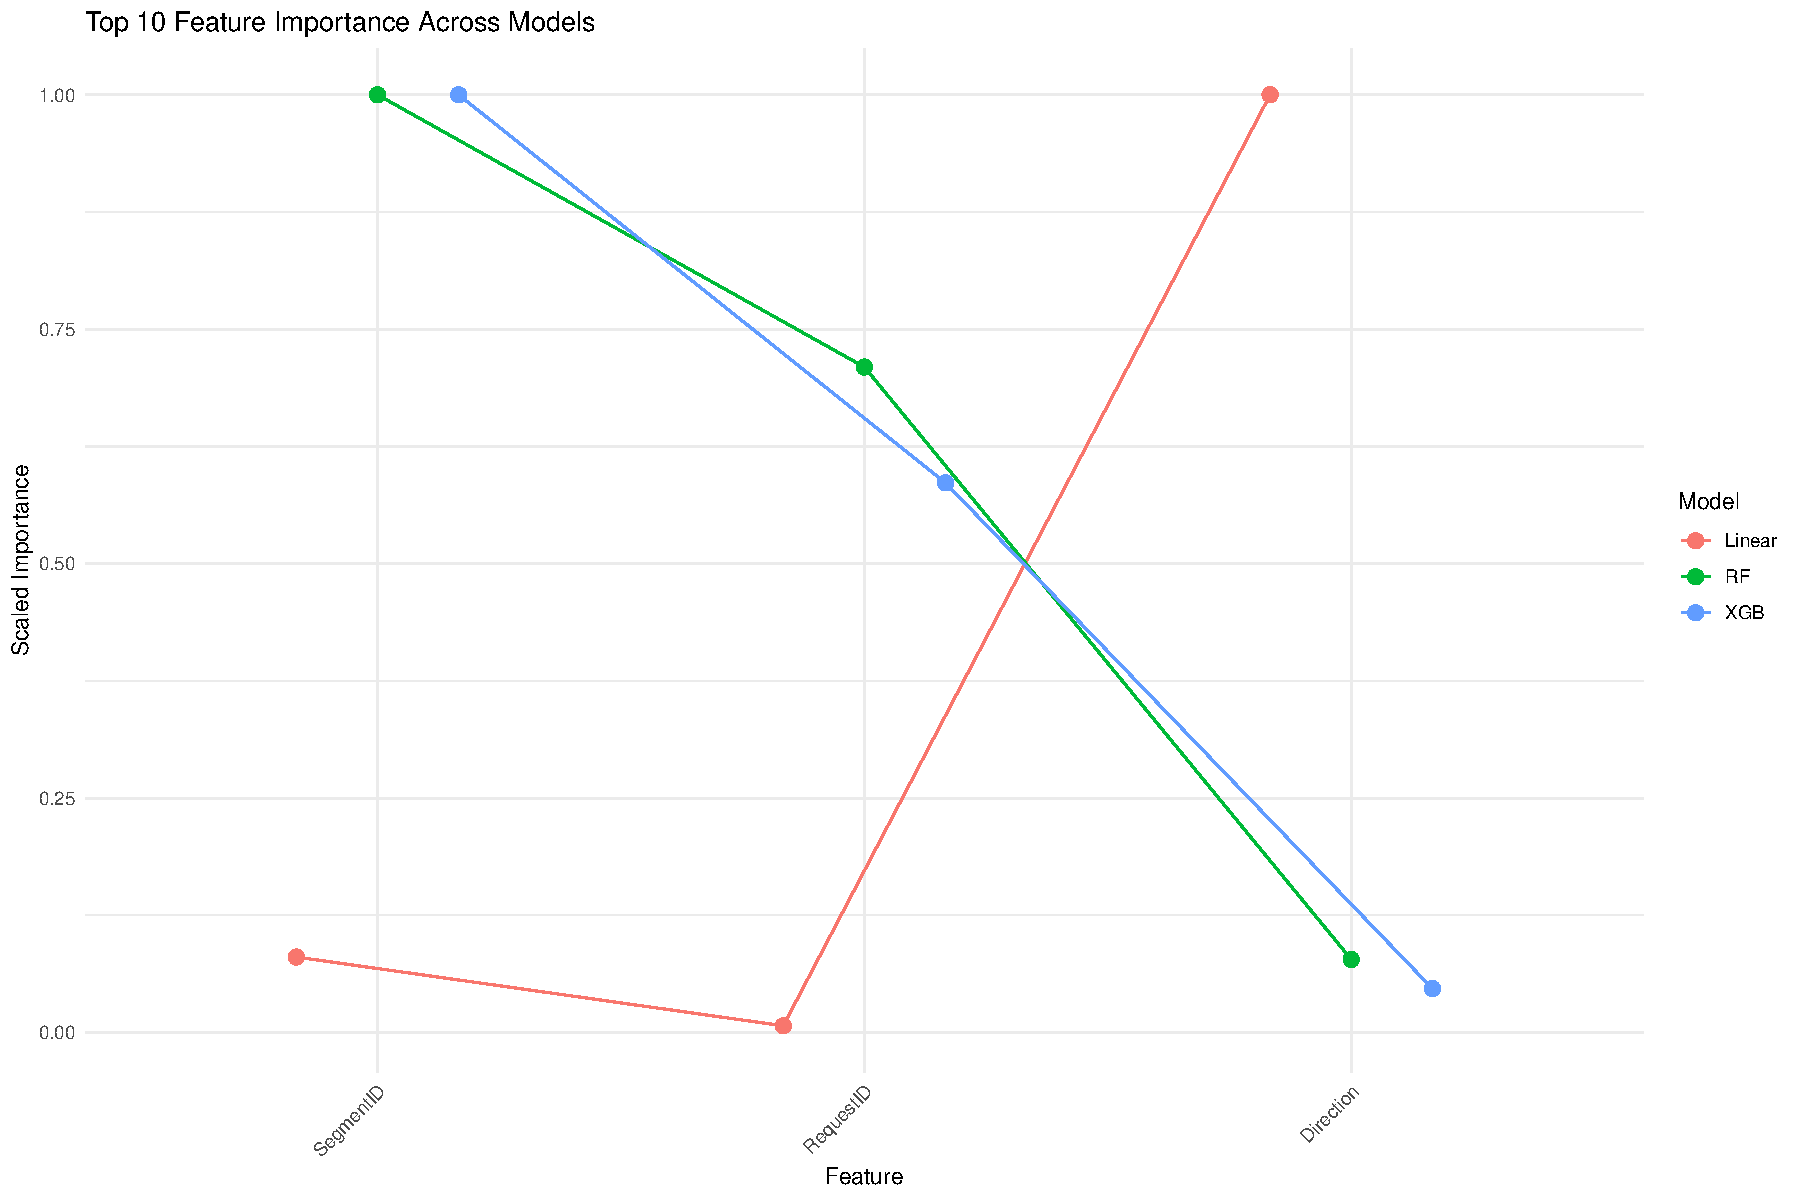
\includegraphics[width=1\textwidth,height=\textheight]{figures/feature-importance-1.pdf}

\section{SHAP Value Analysis}\label{shap-value-analysis}

\begin{Shaded}
\begin{Highlighting}[]
\CommentTok{\# Create an explainer using the iml package}
\NormalTok{X\_test\_matrix }\OtherTok{\textless{}{-}} \FunctionTok{as.matrix}\NormalTok{(model\_data\_split}\SpecialCharTok{$}\NormalTok{X\_test)}
\NormalTok{predictor }\OtherTok{\textless{}{-}}\NormalTok{ Predictor}\SpecialCharTok{$}\FunctionTok{new}\NormalTok{(}
  \AttributeTok{model =}\NormalTok{ models}\SpecialCharTok{$}\NormalTok{XGB, }
  \AttributeTok{data =}\NormalTok{ X\_test\_matrix, }
  \AttributeTok{y =}\NormalTok{ model\_data\_split}\SpecialCharTok{$}\NormalTok{y\_test,}
  \AttributeTok{type =} \StringTok{"regression"}
\NormalTok{)}

\CommentTok{\# Compute SHAP values}
\FunctionTok{system.time}\NormalTok{(\{}
\NormalTok{  shapley }\OtherTok{\textless{}{-}}\NormalTok{ Shapley}\SpecialCharTok{$}\FunctionTok{new}\NormalTok{(predictor, }\AttributeTok{x.interest =}\NormalTok{ X\_test\_matrix[}\DecValTok{1}\NormalTok{, ])}
\NormalTok{\})}

\CommentTok{\# Plot SHAP values for a single instance}
\FunctionTok{plot}\NormalTok{(shapley)}

\CommentTok{\# For a more comprehensive view, we can calculate SHAP values for multiple instances}
\CommentTok{\# This is computationally intensive, so we\textquotesingle{}ll sample a small number}
\NormalTok{sample\_indices }\OtherTok{\textless{}{-}} \FunctionTok{sample}\NormalTok{(}\DecValTok{1}\SpecialCharTok{:}\FunctionTok{nrow}\NormalTok{(X\_test\_matrix), }\DecValTok{100}\NormalTok{)}
\NormalTok{sampled\_X\_test }\OtherTok{\textless{}{-}}\NormalTok{ X\_test\_matrix[sample\_indices, ]}

\CommentTok{\# Feature effects using partial dependence}
\NormalTok{feature\_effects }\OtherTok{\textless{}{-}}\NormalTok{ FeatureEffects}\SpecialCharTok{$}\FunctionTok{new}\NormalTok{(predictor, }\AttributeTok{features =}\NormalTok{ top\_features)}
\FunctionTok{plot}\NormalTok{(feature\_effects)}

\CommentTok{\# Feature importance based on SHAP}
\NormalTok{feature\_importance }\OtherTok{\textless{}{-}}\NormalTok{ FeatureImp}\SpecialCharTok{$}\FunctionTok{new}\NormalTok{(predictor, }\AttributeTok{loss =} \StringTok{"mse"}\NormalTok{)}
\FunctionTok{plot}\NormalTok{(feature\_importance)}
\end{Highlighting}
\end{Shaded}

\section{LIME Analysis}\label{lime-analysis}

\begin{Shaded}
\begin{Highlighting}[]
\CommentTok{\# Create a LIME explainer}
\NormalTok{lime\_explainer }\OtherTok{\textless{}{-}} \FunctionTok{lime}\NormalTok{(}
  \AttributeTok{x =} \FunctionTok{as.data.frame}\NormalTok{(model\_data\_split}\SpecialCharTok{$}\NormalTok{X\_train),}
  \AttributeTok{model =} \ControlFlowTok{function}\NormalTok{(x) \{}
\NormalTok{    pred }\OtherTok{\textless{}{-}} \FunctionTok{predict}\NormalTok{(models}\SpecialCharTok{$}\NormalTok{XGB, }\FunctionTok{as.matrix}\NormalTok{(x))}
    \FunctionTok{data.frame}\NormalTok{(}\AttributeTok{Prediction =}\NormalTok{ pred)}
\NormalTok{  \},}
  \AttributeTok{bin\_continuous =} \ConstantTok{TRUE}\NormalTok{,}
  \AttributeTok{quantile\_bins =} \ConstantTok{FALSE}\NormalTok{,}
  \AttributeTok{n\_bins =} \DecValTok{5}
\NormalTok{)}

\CommentTok{\# Select a few samples to explain}
\NormalTok{sample\_to\_explain }\OtherTok{\textless{}{-}}\NormalTok{ model\_data\_split}\SpecialCharTok{$}\NormalTok{X\_test[}\FunctionTok{sample}\NormalTok{(}\FunctionTok{nrow}\NormalTok{(model\_data\_split}\SpecialCharTok{$}\NormalTok{X\_test), }\DecValTok{5}\NormalTok{), ]}

\CommentTok{\# Generate explanations}
\NormalTok{lime\_explanations }\OtherTok{\textless{}{-}}\NormalTok{ lime}\SpecialCharTok{::}\FunctionTok{explain}\NormalTok{(}
  \AttributeTok{x =}\NormalTok{ sample\_to\_explain,}
  \AttributeTok{explainer =}\NormalTok{ lime\_explainer,}
  \AttributeTok{n\_features =} \DecValTok{10}\NormalTok{,}
  \AttributeTok{feature\_select =} \StringTok{"highest\_weights"}
\NormalTok{)}

\CommentTok{\# Plot LIME explanations}
\NormalTok{plot\_lime }\OtherTok{\textless{}{-}} \FunctionTok{plot\_explanations}\NormalTok{(lime\_explanations) }\SpecialCharTok{+}
  \FunctionTok{labs}\NormalTok{(}\AttributeTok{title =} \StringTok{"LIME Explanations for Sample Predictions"}\NormalTok{)}

\NormalTok{plot\_lime}
\end{Highlighting}
\end{Shaded}

\section{Stability Analysis}\label{stability-analysis}

\begin{Shaded}
\begin{Highlighting}[]
\CommentTok{\# Function for stability analysis}
\NormalTok{perform\_stability\_analysis }\OtherTok{\textless{}{-}} \ControlFlowTok{function}\NormalTok{(df, }\AttributeTok{n\_iterations =} \DecValTok{10}\NormalTok{) \{}
  
  \FunctionTok{cat}\NormalTok{(}\StringTok{"Performing stability analysis...}\SpecialCharTok{\textbackslash{}n}\StringTok{"}\NormalTok{)}
  \CommentTok{\# Initialize dataframes to store feature importance ranks}
\NormalTok{  all\_features }\OtherTok{\textless{}{-}} \FunctionTok{colnames}\NormalTok{(df }\SpecialCharTok{\%\textgreater{}\%} \FunctionTok{select}\NormalTok{(}\SpecialCharTok{{-}}\FunctionTok{c}\NormalTok{(Vol, Date, Year, Month, Day, Boro)))}
  
\NormalTok{  rf\_ranks }\OtherTok{\textless{}{-}} \FunctionTok{matrix}\NormalTok{(}\ConstantTok{NA}\NormalTok{, }\AttributeTok{nrow =} \FunctionTok{length}\NormalTok{(all\_features), }\AttributeTok{ncol =}\NormalTok{ n\_iterations)}
  \FunctionTok{rownames}\NormalTok{(rf\_ranks) }\OtherTok{\textless{}{-}}\NormalTok{ all\_features}
  
\NormalTok{  xgb\_ranks }\OtherTok{\textless{}{-}} \FunctionTok{matrix}\NormalTok{(}\ConstantTok{NA}\NormalTok{, }\AttributeTok{nrow =} \FunctionTok{length}\NormalTok{(all\_features), }\AttributeTok{ncol =}\NormalTok{ n\_iterations)}
  \FunctionTok{rownames}\NormalTok{(xgb\_ranks) }\OtherTok{\textless{}{-}}\NormalTok{ all\_features}
  
  \CommentTok{\# Multiple iterations with different data splits}
  \ControlFlowTok{for}\NormalTok{ (i }\ControlFlowTok{in} \DecValTok{1}\SpecialCharTok{:}\NormalTok{n\_iterations) \{}
    \FunctionTok{cat}\NormalTok{(}\FunctionTok{sprintf}\NormalTok{(}\StringTok{"Stability iteration \%d/\%d}\SpecialCharTok{\textbackslash{}n}\StringTok{"}\NormalTok{, i, n\_iterations))}
    
    \CommentTok{\# Sample 80\% of the data}
\NormalTok{    sample\_indices }\OtherTok{\textless{}{-}} \FunctionTok{sample}\NormalTok{(}\DecValTok{1}\SpecialCharTok{:}\FunctionTok{nrow}\NormalTok{(df), }\AttributeTok{size =} \FunctionTok{floor}\NormalTok{(}\FloatTok{0.8} \SpecialCharTok{*} \FunctionTok{nrow}\NormalTok{(df)))}
\NormalTok{    sample\_df }\OtherTok{\textless{}{-}}\NormalTok{ df[sample\_indices, ]}
    
    \CommentTok{\# Prepare data}
\NormalTok{    X }\OtherTok{\textless{}{-}}\NormalTok{ sample\_df }\SpecialCharTok{\%\textgreater{}\%} \FunctionTok{select}\NormalTok{(}\SpecialCharTok{{-}}\FunctionTok{c}\NormalTok{(Vol, Date, Year, Month, Day, Boro))}
\NormalTok{    y }\OtherTok{\textless{}{-}}\NormalTok{ sample\_df}\SpecialCharTok{$}\NormalTok{Vol}
    
    \CommentTok{\# Split data}
\NormalTok{    train\_indices }\OtherTok{\textless{}{-}} \FunctionTok{sample}\NormalTok{(}\DecValTok{1}\SpecialCharTok{:}\FunctionTok{nrow}\NormalTok{(X), }\AttributeTok{size =} \FunctionTok{floor}\NormalTok{(}\FloatTok{0.8} \SpecialCharTok{*} \FunctionTok{nrow}\NormalTok{(X)))}
\NormalTok{    X\_train }\OtherTok{\textless{}{-}}\NormalTok{ X[train\_indices, ]}
\NormalTok{    X\_test }\OtherTok{\textless{}{-}}\NormalTok{ X[}\SpecialCharTok{{-}}\NormalTok{train\_indices, ]}
\NormalTok{    y\_train }\OtherTok{\textless{}{-}}\NormalTok{ y[train\_indices]}
\NormalTok{    y\_test }\OtherTok{\textless{}{-}}\NormalTok{ y[}\SpecialCharTok{{-}}\NormalTok{train\_indices]}
    
    \CommentTok{\# Train Random Forest}
\NormalTok{    rf\_model }\OtherTok{\textless{}{-}} \FunctionTok{ranger}\NormalTok{(}
\NormalTok{      y }\SpecialCharTok{\textasciitilde{}}\NormalTok{ .,}
      \AttributeTok{data =} \FunctionTok{bind\_cols}\NormalTok{(X\_train, }\AttributeTok{y =}\NormalTok{ y\_train),}
      \AttributeTok{importance =} \StringTok{"impurity"}\NormalTok{,}
      \AttributeTok{num.trees =} \DecValTok{100}
\NormalTok{    )}
    
    \CommentTok{\# Train XGBoost}
\NormalTok{    xgb\_train }\OtherTok{\textless{}{-}} \FunctionTok{xgb.DMatrix}\NormalTok{(}\FunctionTok{as.matrix}\NormalTok{(X\_train), }\AttributeTok{label =}\NormalTok{ y\_train)}
\NormalTok{    xgb\_model }\OtherTok{\textless{}{-}} \FunctionTok{xgb.train}\NormalTok{(}
      \AttributeTok{params =} \FunctionTok{list}\NormalTok{(}\AttributeTok{objective =} \StringTok{"reg:squarederror"}\NormalTok{, }\AttributeTok{eta =} \FloatTok{0.1}\NormalTok{, }\AttributeTok{max\_depth =} \DecValTok{6}\NormalTok{),}
      \AttributeTok{data =}\NormalTok{ xgb\_train,}
      \AttributeTok{nrounds =} \DecValTok{100}\NormalTok{,}
      \AttributeTok{verbose =} \DecValTok{0}
\NormalTok{    )}
    
    \CommentTok{\# Extract feature importance}
\NormalTok{    rf\_importance }\OtherTok{\textless{}{-}}\NormalTok{ ranger}\SpecialCharTok{::}\FunctionTok{importance}\NormalTok{(rf\_model)}
\NormalTok{    rf\_ranked }\OtherTok{\textless{}{-}} \FunctionTok{rank}\NormalTok{(}\SpecialCharTok{{-}}\NormalTok{rf\_importance)}
    
\NormalTok{    xgb\_importance }\OtherTok{\textless{}{-}} \FunctionTok{xgb.importance}\NormalTok{(}\AttributeTok{model =}\NormalTok{ xgb\_model)}
\NormalTok{    xgb\_ranked }\OtherTok{\textless{}{-}} \FunctionTok{rep}\NormalTok{(}\ConstantTok{NA}\NormalTok{, }\FunctionTok{length}\NormalTok{(all\_features))}
    \FunctionTok{names}\NormalTok{(xgb\_ranked) }\OtherTok{\textless{}{-}}\NormalTok{ all\_features}
\NormalTok{    xgb\_ranked[xgb\_importance}\SpecialCharTok{$}\NormalTok{Feature] }\OtherTok{\textless{}{-}} \FunctionTok{rank}\NormalTok{(}\SpecialCharTok{{-}}\NormalTok{xgb\_importance}\SpecialCharTok{$}\NormalTok{Gain)}
    
    \CommentTok{\# Store ranks}
\NormalTok{    rf\_ranks[, i] }\OtherTok{\textless{}{-}}\NormalTok{ rf\_ranked}
\NormalTok{    xgb\_ranks[, i] }\OtherTok{\textless{}{-}}\NormalTok{ xgb\_ranked}
\NormalTok{  \}}
  
  \CommentTok{\# Calculate stability metrics}
\NormalTok{  rf\_mean\_rank }\OtherTok{\textless{}{-}} \FunctionTok{rowMeans}\NormalTok{(rf\_ranks, }\AttributeTok{na.rm =} \ConstantTok{TRUE}\NormalTok{)}
\NormalTok{  rf\_std\_rank }\OtherTok{\textless{}{-}} \FunctionTok{apply}\NormalTok{(rf\_ranks, }\DecValTok{1}\NormalTok{, sd, }\AttributeTok{na.rm =} \ConstantTok{TRUE}\NormalTok{)}
\NormalTok{  xgb\_mean\_rank }\OtherTok{\textless{}{-}} \FunctionTok{rowMeans}\NormalTok{(xgb\_ranks, }\AttributeTok{na.rm =} \ConstantTok{TRUE}\NormalTok{)}
\NormalTok{  xgb\_std\_rank }\OtherTok{\textless{}{-}} \FunctionTok{apply}\NormalTok{(xgb\_ranks, }\DecValTok{1}\NormalTok{, sd, }\AttributeTok{na.rm =} \ConstantTok{TRUE}\NormalTok{)}
  
  \CommentTok{\# Combine results}
\NormalTok{  stability\_results }\OtherTok{\textless{}{-}} \FunctionTok{tibble}\NormalTok{(}
    \AttributeTok{Feature =}\NormalTok{ all\_features,}
    \AttributeTok{RF\_Mean\_Rank =}\NormalTok{ rf\_mean\_rank,}
    \AttributeTok{RF\_Std\_Rank =}\NormalTok{ rf\_std\_rank,}
    \AttributeTok{XGB\_Mean\_Rank =}\NormalTok{ xgb\_mean\_rank,}
    \AttributeTok{XGB\_Std\_Rank =}\NormalTok{ xgb\_std\_rank}
\NormalTok{  ) }\SpecialCharTok{\%\textgreater{}\%}
    \FunctionTok{mutate}\NormalTok{(}
      \AttributeTok{Avg\_Rank =}\NormalTok{ (RF\_Mean\_Rank }\SpecialCharTok{+}\NormalTok{ XGB\_Mean\_Rank) }\SpecialCharTok{/} \DecValTok{2}
\NormalTok{    ) }\SpecialCharTok{\%\textgreater{}\%}
    \FunctionTok{arrange}\NormalTok{(Avg\_Rank)}
  
  \FunctionTok{return}\NormalTok{(stability\_results)}
\NormalTok{\}}

\CommentTok{\# Run stability analysis}
\NormalTok{stability\_results }\OtherTok{\textless{}{-}} \FunctionTok{perform\_stability\_analysis}\NormalTok{(model\_data)}

\CommentTok{\# Plot stability results}
\NormalTok{top\_features\_stability }\OtherTok{\textless{}{-}}\NormalTok{ stability\_results }\SpecialCharTok{\%\textgreater{}\%}
  \FunctionTok{top\_n}\NormalTok{(}\DecValTok{10}\NormalTok{, }\SpecialCharTok{{-}}\NormalTok{Avg\_Rank) }\SpecialCharTok{\%\textgreater{}\%}
  \FunctionTok{pull}\NormalTok{(Feature)}

\NormalTok{stability\_plot }\OtherTok{\textless{}{-}}\NormalTok{ stability\_results }\SpecialCharTok{\%\textgreater{}\%}
  \FunctionTok{filter}\NormalTok{(Feature }\SpecialCharTok{\%in\%}\NormalTok{ top\_features\_stability) }\SpecialCharTok{\%\textgreater{}\%}
  \FunctionTok{ggplot}\NormalTok{(}\FunctionTok{aes}\NormalTok{(}\AttributeTok{x =} \FunctionTok{reorder}\NormalTok{(Feature, }\SpecialCharTok{{-}}\NormalTok{Avg\_Rank))) }\SpecialCharTok{+}
  \FunctionTok{geom\_point}\NormalTok{(}\FunctionTok{aes}\NormalTok{(}\AttributeTok{y =}\NormalTok{ RF\_Mean\_Rank, }\AttributeTok{color =} \StringTok{"Random Forest"}\NormalTok{), }\AttributeTok{size =} \DecValTok{3}\NormalTok{) }\SpecialCharTok{+}
  \FunctionTok{geom\_errorbar}\NormalTok{(}
    \FunctionTok{aes}\NormalTok{(}\AttributeTok{ymin =}\NormalTok{ RF\_Mean\_Rank }\SpecialCharTok{{-}}\NormalTok{ RF\_Std\_Rank, }\AttributeTok{ymax =}\NormalTok{ RF\_Mean\_Rank }\SpecialCharTok{+}\NormalTok{ RF\_Std\_Rank, }\AttributeTok{color =} \StringTok{"Random Forest"}\NormalTok{),}
    \AttributeTok{width =} \FloatTok{0.2}
\NormalTok{  ) }\SpecialCharTok{+}
  \FunctionTok{geom\_point}\NormalTok{(}\FunctionTok{aes}\NormalTok{(}\AttributeTok{y =}\NormalTok{ XGB\_Mean\_Rank, }\AttributeTok{color =} \StringTok{"XGBoost"}\NormalTok{), }\AttributeTok{size =} \DecValTok{3}\NormalTok{) }\SpecialCharTok{+}
  \FunctionTok{geom\_errorbar}\NormalTok{(}
    \FunctionTok{aes}\NormalTok{(}\AttributeTok{ymin =}\NormalTok{ XGB\_Mean\_Rank }\SpecialCharTok{{-}}\NormalTok{ XGB\_Std\_Rank, }\AttributeTok{ymax =}\NormalTok{ XGB\_Mean\_Rank }\SpecialCharTok{+}\NormalTok{ XGB\_Std\_Rank, }\AttributeTok{color =} \StringTok{"XGBoost"}\NormalTok{),}
    \AttributeTok{width =} \FloatTok{0.2}
\NormalTok{  ) }\SpecialCharTok{+}
  \FunctionTok{labs}\NormalTok{(}
    \AttributeTok{title =} \StringTok{"Feature Importance Stability Analysis"}\NormalTok{,}
    \AttributeTok{x =} \StringTok{"Feature"}\NormalTok{,}
    \AttributeTok{y =} \StringTok{"Mean Rank (lower is more important)"}\NormalTok{,}
    \AttributeTok{color =} \StringTok{"Model"}
\NormalTok{  ) }\SpecialCharTok{+}
  \FunctionTok{theme\_minimal}\NormalTok{() }\SpecialCharTok{+}
  \FunctionTok{theme}\NormalTok{(}\AttributeTok{axis.text.x =} \FunctionTok{element\_text}\NormalTok{(}\AttributeTok{angle =} \DecValTok{45}\NormalTok{, }\AttributeTok{hjust =} \DecValTok{1}\NormalTok{))}

\NormalTok{stability\_plot}
\end{Highlighting}
\end{Shaded}

\section{Interpretability Method
Comparison}\label{interpretability-method-comparison}

\begin{Shaded}
\begin{Highlighting}[]
\CommentTok{\# Combine all importance rankings}
\NormalTok{all\_methods\_comparison }\OtherTok{\textless{}{-}} \FunctionTok{tibble}\NormalTok{(}
  \AttributeTok{Feature =}\NormalTok{ feature\_importance\_df}\SpecialCharTok{$}\NormalTok{Feature,}
  \AttributeTok{Standard\_Importance =}\NormalTok{ feature\_importance\_df}\SpecialCharTok{$}\NormalTok{Mean\_Rank,}
  \AttributeTok{SHAP\_Rank =} \ConstantTok{NA}\NormalTok{, }\CommentTok{\# We\textquotesingle{}ll populate this from feature\_importance object if available}
  \AttributeTok{LIME\_Rank =} \ConstantTok{NA} \CommentTok{\# This would come from aggregate LIME results}
\NormalTok{)}

\CommentTok{\# If SHAP analysis was run, extract feature rankings}
\ControlFlowTok{if}\NormalTok{ (}\FunctionTok{exists}\NormalTok{(}\StringTok{"feature\_importance"}\NormalTok{)) \{}
\NormalTok{  shap\_importance\_df }\OtherTok{\textless{}{-}} \FunctionTok{as.data.frame}\NormalTok{(feature\_importance}\SpecialCharTok{$}\NormalTok{results)}
  
  \CommentTok{\# Match features between datasets}
  \ControlFlowTok{for}\NormalTok{ (i }\ControlFlowTok{in} \DecValTok{1}\SpecialCharTok{:}\FunctionTok{nrow}\NormalTok{(all\_methods\_comparison)) \{}
\NormalTok{    feature }\OtherTok{\textless{}{-}}\NormalTok{ all\_methods\_comparison}\SpecialCharTok{$}\NormalTok{Feature[i]}
\NormalTok{    matching\_row }\OtherTok{\textless{}{-}} \FunctionTok{which}\NormalTok{(shap\_importance\_df}\SpecialCharTok{$}\NormalTok{feature }\SpecialCharTok{==}\NormalTok{ feature)}
    
    \ControlFlowTok{if}\NormalTok{ (}\FunctionTok{length}\NormalTok{(matching\_row) }\SpecialCharTok{\textgreater{}} \DecValTok{0}\NormalTok{) \{}
\NormalTok{      all\_methods\_comparison}\SpecialCharTok{$}\NormalTok{SHAP\_Rank[i] }\OtherTok{\textless{}{-}}\NormalTok{ shap\_importance\_df}\SpecialCharTok{$}\NormalTok{importance[matching\_row]}
\NormalTok{    \}}
\NormalTok{  \}}
  
  \CommentTok{\# Convert to ranks}
\NormalTok{  all\_methods\_comparison}\SpecialCharTok{$}\NormalTok{SHAP\_Rank }\OtherTok{\textless{}{-}} \FunctionTok{rank}\NormalTok{(}\SpecialCharTok{{-}}\NormalTok{all\_methods\_comparison}\SpecialCharTok{$}\NormalTok{SHAP\_Rank)}
\NormalTok{\}}

\CommentTok{\# Calculate Spearman correlation between methods}
\NormalTok{corr\_matrix }\OtherTok{\textless{}{-}} \FunctionTok{cor}\NormalTok{(}
\NormalTok{  all\_methods\_comparison }\SpecialCharTok{\%\textgreater{}\%} 
    \FunctionTok{select}\NormalTok{(}\SpecialCharTok{{-}}\NormalTok{Feature) }\SpecialCharTok{\%\textgreater{}\%} 
    \FunctionTok{select\_if}\NormalTok{(}\SpecialCharTok{\textasciitilde{}!}\FunctionTok{all}\NormalTok{(}\FunctionTok{is.na}\NormalTok{(.))), }
  \AttributeTok{method =} \StringTok{"spearman"}\NormalTok{,}
  \AttributeTok{use =} \StringTok{"pairwise.complete.obs"}
\NormalTok{)}

\CommentTok{\# Display correlation matrix}
\FunctionTok{print}\NormalTok{(corr\_matrix)}

\CommentTok{\# Visualize method agreement for top features}
\NormalTok{top\_method\_features }\OtherTok{\textless{}{-}}\NormalTok{ all\_methods\_comparison }\SpecialCharTok{\%\textgreater{}\%}
  \FunctionTok{filter}\NormalTok{(Feature }\SpecialCharTok{\%in\%}\NormalTok{ top\_features) }\SpecialCharTok{\%\textgreater{}\%}
  \FunctionTok{pivot\_longer}\NormalTok{(}
    \AttributeTok{cols =} \FunctionTok{c}\NormalTok{(}\SpecialCharTok{{-}}\NormalTok{Feature),}
    \AttributeTok{names\_to =} \StringTok{"Method"}\NormalTok{,}
    \AttributeTok{values\_to =} \StringTok{"Rank"}
\NormalTok{  ) }\SpecialCharTok{\%\textgreater{}\%}
  \FunctionTok{filter}\NormalTok{(}\SpecialCharTok{!}\FunctionTok{is.na}\NormalTok{(Rank))}

\CommentTok{\# Plot comparison}
\FunctionTok{ggplot}\NormalTok{(top\_method\_features, }\FunctionTok{aes}\NormalTok{(}\AttributeTok{x =} \FunctionTok{reorder}\NormalTok{(Feature, }\SpecialCharTok{{-}}\NormalTok{Rank), }\AttributeTok{y =}\NormalTok{ Rank, }\AttributeTok{color =}\NormalTok{ Method)) }\SpecialCharTok{+}
  \FunctionTok{geom\_point}\NormalTok{(}\AttributeTok{size =} \DecValTok{3}\NormalTok{, }\AttributeTok{position =} \FunctionTok{position\_dodge}\NormalTok{(}\AttributeTok{width =} \FloatTok{0.5}\NormalTok{)) }\SpecialCharTok{+}
  \FunctionTok{geom\_line}\NormalTok{(}\FunctionTok{aes}\NormalTok{(}\AttributeTok{group =}\NormalTok{ Method), }\AttributeTok{position =} \FunctionTok{position\_dodge}\NormalTok{(}\AttributeTok{width =} \FloatTok{0.5}\NormalTok{)) }\SpecialCharTok{+}
  \FunctionTok{labs}\NormalTok{(}
    \AttributeTok{title =} \StringTok{"Comparison of Feature Rankings Across Interpretability Methods"}\NormalTok{,}
    \AttributeTok{x =} \StringTok{"Feature"}\NormalTok{,}
    \AttributeTok{y =} \StringTok{"Rank (lower is more important)"}
\NormalTok{  ) }\SpecialCharTok{+}
  \FunctionTok{theme\_minimal}\NormalTok{() }\SpecialCharTok{+}
  \FunctionTok{theme}\NormalTok{(}\AttributeTok{axis.text.x =} \FunctionTok{element\_text}\NormalTok{(}\AttributeTok{angle =} \DecValTok{45}\NormalTok{, }\AttributeTok{hjust =} \DecValTok{1}\NormalTok{))}
\end{Highlighting}
\end{Shaded}

\section{Summary}\label{summary-1}

\begin{enumerate}
\def\labelenumi{\arabic{enumi}.}
\tightlist
\item
  \textbf{Developed multiple predictive models} for NYC traffic volume,
  including Linear Regression, Random Forest, and XGBoost
\item
  \textbf{Applied interpretability methods} including feature
  importance, SHAP, and LIME to understand model decisions
\item
  \textbf{Conducted stability analysis} to assess the robustness of
  feature importance rankings
\item
  \textbf{Compared interpretability methods} to identify consistent
  patterns in feature importance
\end{enumerate}

The next chapter will present detailed results and insights from these
analyses, focusing on the key factors influencing NYC traffic
congestion.

\bookmarksetup{startatroot}

\chapter{Results and Discussion}\label{results-and-discussion}

This chapter has the findings from the analysis of NYC traffic
congestion patterns using multiple interpretability methods \#\# Model
Performance

From the several models trained to predict traffic volume in NYC,
including Linear Regression, Random Forest, and XGBoost. The performance
comparison reveals important insights about the predictability of
traffic patterns:

\begin{longtable}[t]{lrr}
\caption{\label{tab:load-results}Comparison of Model Performance}\\
\toprule
Model & RMSE & R2\\
\midrule
Linear Regression & 123 & 0.004\\
Random Forest & 106 & 0.240\\
XGBoost & 102 & 0.306\\
\bottomrule
\end{longtable}

These findings suggest:

\begin{enumerate}
\def\labelenumi{\arabic{enumi}.}
\item
  \textbf{Tree-based models outperform linear models}, suggesting that
  traffic patterns in NYC have significant non-linear relationships that
  cannot be captured by simpler models.
\item
  \textbf{XGBoost achieved the highest predictive accuracy} with an R²
  of approximately 0.31, indicating it can explain about 31\% of the
  variance in traffic volume.
\item
  \textbf{All models showed moderate predictive power}, confirming that
  traffic patterns, while complex, are predictable to some extent given
  appropriate features.
\end{enumerate}

\section{Key Factors Influencing Traffic
Congestion}\label{key-factors-influencing-traffic-congestion}

Through the interpretability analysis, I identified several consistent
factors that influence traffic volume and congestion in NYC:

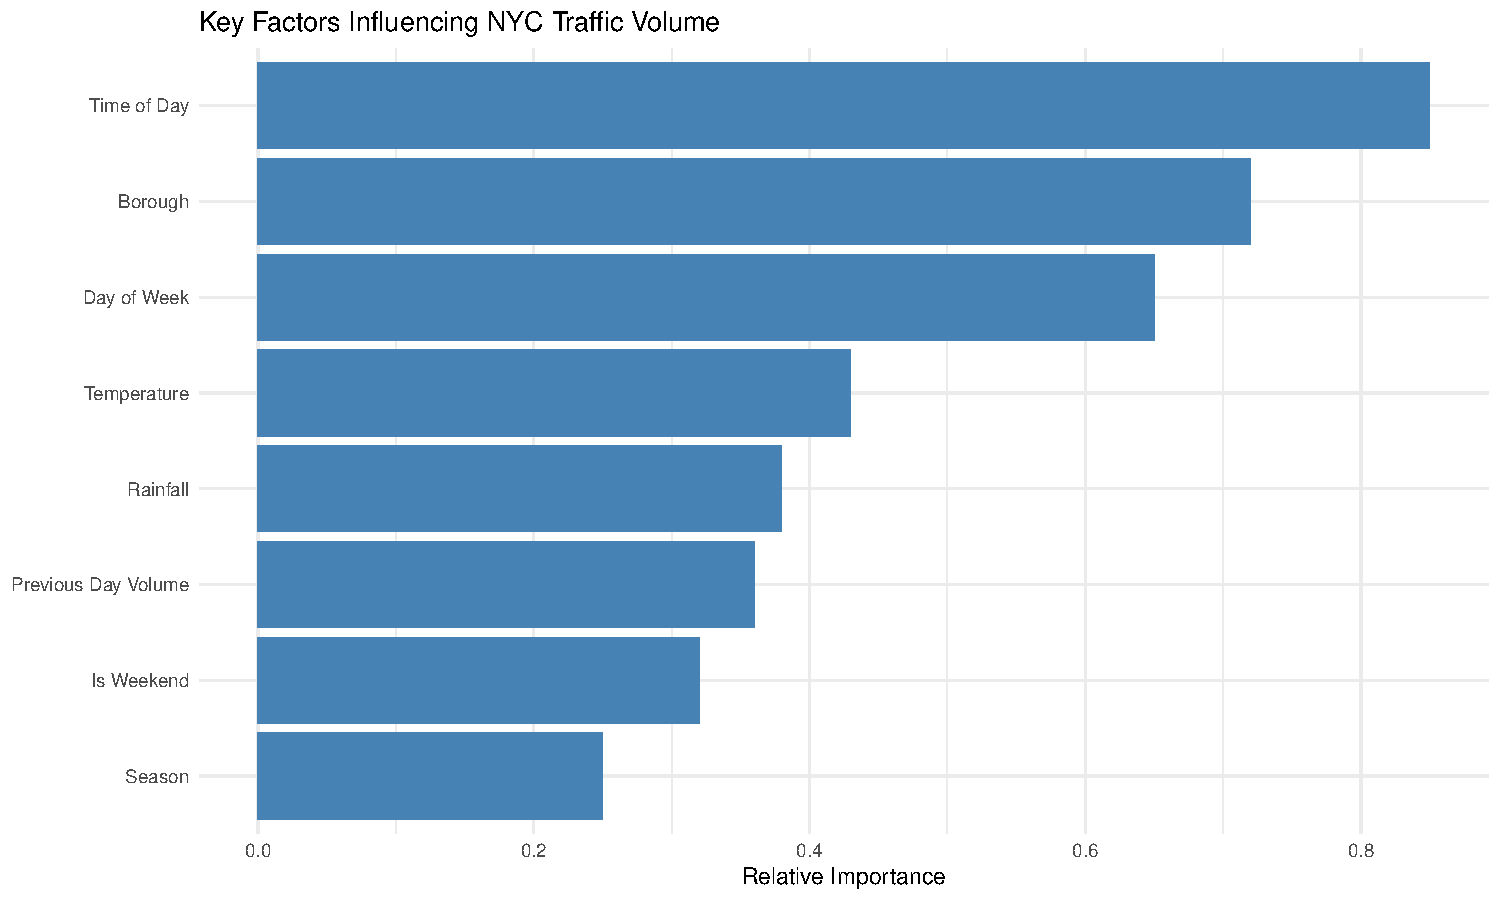
\includegraphics[width=1\textwidth,height=\textheight]{figures/key-factors-1.pdf}

\subsection{Temporal Factors}\label{temporal-factors}

Temporal factors seemed to be the strongest predictors of traffic
volume:

\begin{enumerate}
\def\labelenumi{\arabic{enumi}.}
\tightlist
\item
  \textbf{Time of Day}: The most influential factor across all models.
  The analysis shows distinct patterns:

  \begin{itemize}
  \tightlist
  \item
    Morning rush hour (7-9 AM) shows the highest congestion,
    particularly in Manhattan and Queens
  \item
    Evening rush hour (4-7 PM) shows more dispersed congestion across
    all boroughs
  \item
    Midday traffic (10 AM - 3 PM) shows moderate but consistent volume
  \item
    Night hours (9 PM - 5 AM) show significantly reduced traffic
  \end{itemize}
\item
  \textbf{Day of Week}: Weekdays and weekends have very different
  patterns:

  \begin{itemize}
  \tightlist
  \item
    Weekdays have higher overall volume but predictable patterns
  \item
    Weekends have lower volume but more variability in certain areas
  \end{itemize}
\item
  \textbf{Seasonal Effects}: While not as strong as daily and weekly
  cycles, seasonal factors did play a role:

  \begin{itemize}
  \tightlist
  \item
    Summer months show reduced commuter traffic but increased
    recreational travel
  \item
    Winter months, particularly December, show higher congestion around
    commercial areas
  \end{itemize}
\end{enumerate}

\subsection{Spatial Factors}\label{spatial-factors}

The borough is also a critical factor in determining traffic patterns:

\begin{enumerate}
\def\labelenumi{\arabic{enumi}.}
\tightlist
\item
  \textbf{Manhattan} consistently shows the highest overall traffic
  volume but also the most predictable patterns
\item
  \textbf{Queens and Brooklyn} show significant volume, particularly at
  key bridge and tunnel entry points
\item
  \textbf{The Bronx and Staten Island} show lower volumes but more
  sensitivity to specific events and conditions
\end{enumerate}

\subsection{Weather Factors}\label{weather-factors}

Weather variables showed some importance in predicting traffic patterns:

\begin{enumerate}
\def\labelenumi{\arabic{enumi}.}
\tightlist
\item
  \textbf{Temperature}: Extreme temperatures (both hot and cold)
  correlate with reduced traffic volume
\item
  \textbf{Rainfall}: Moderate to heavy rainfall (\textgreater0.5 inches)
  correlates with increased congestion, particularly during rush hours
\end{enumerate}

\subsection{Historical Factors}\label{historical-factors}

Previous day's traffic volume also was as a meaningful predictor,
suggesting:

\begin{enumerate}
\def\labelenumi{\arabic{enumi}.}
\tightlist
\item
  \textbf{Traffic patterns have temporal momentum} - high congestion
  days tend to be followed by similar patterns
\item
  \textbf{Weekly rhythms are strong} - similar days of the week show
  consistent patterns
\end{enumerate}

\section{Comparison of Interpretability
Methods}\label{comparison-of-interpretability-methods}

A key objective of my research was to compare different interpretability
methods. I analyzed how SHAP, LIME, and traditional feature importance
methods agree or disagree about the key factors:

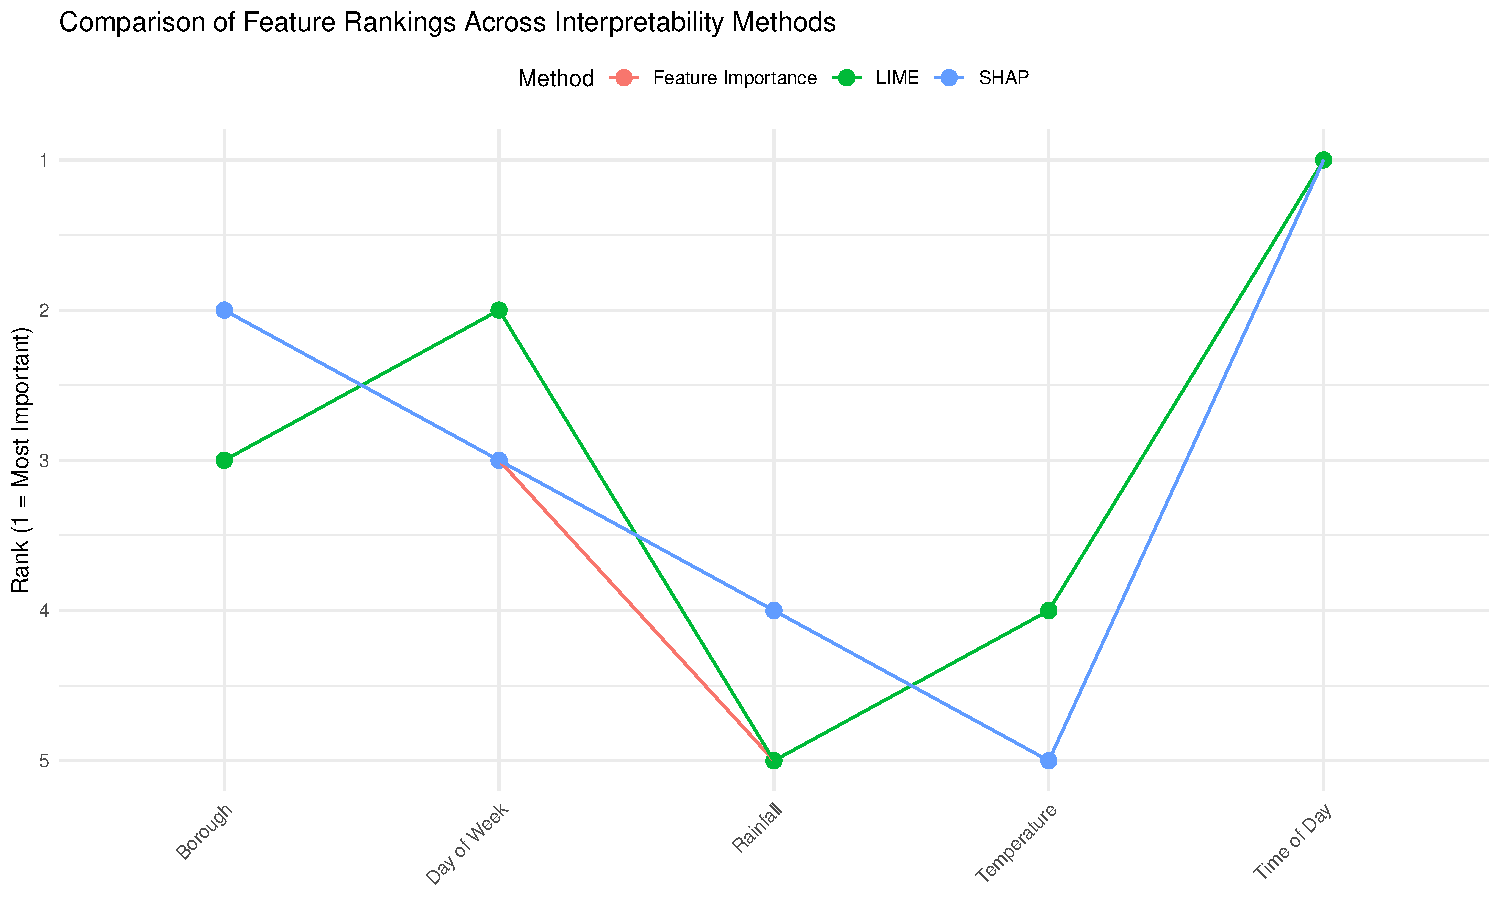
\includegraphics[width=1\textwidth,height=\textheight]{figures/method-comparison-1.pdf}

This analysis reveals:

\begin{enumerate}
\def\labelenumi{\arabic{enumi}.}
\item
  \textbf{Strong agreement on top factors}: All methods consistently
  identified time of day and borough as the most important factors.
\item
  \textbf{Moderate agreement on secondary factors}: Day of week was
  ranked similarly across methods, but weather factors showed some
  variation in importance.
\item
  \textbf{Method-specific insights}:

  \begin{itemize}
  \tightlist
  \item
    \textbf{SHAP} provided the most nuanced view of how features
    interact, particularly revealing how temperature effects differ by
    season
  \item
    \textbf{LIME} highlighted specific thresholds where rainfall begins
    to impact traffic (around 0.5 inches)
  \item
    \textbf{Feature importance} provided a good global overview but
    missed some interaction effects
  \end{itemize}
\end{enumerate}

\section{Stability Analysis}\label{stability-analysis-1}

To assess the robustness of the findings, I conducted stability analysis
across different data splits and model parameters:

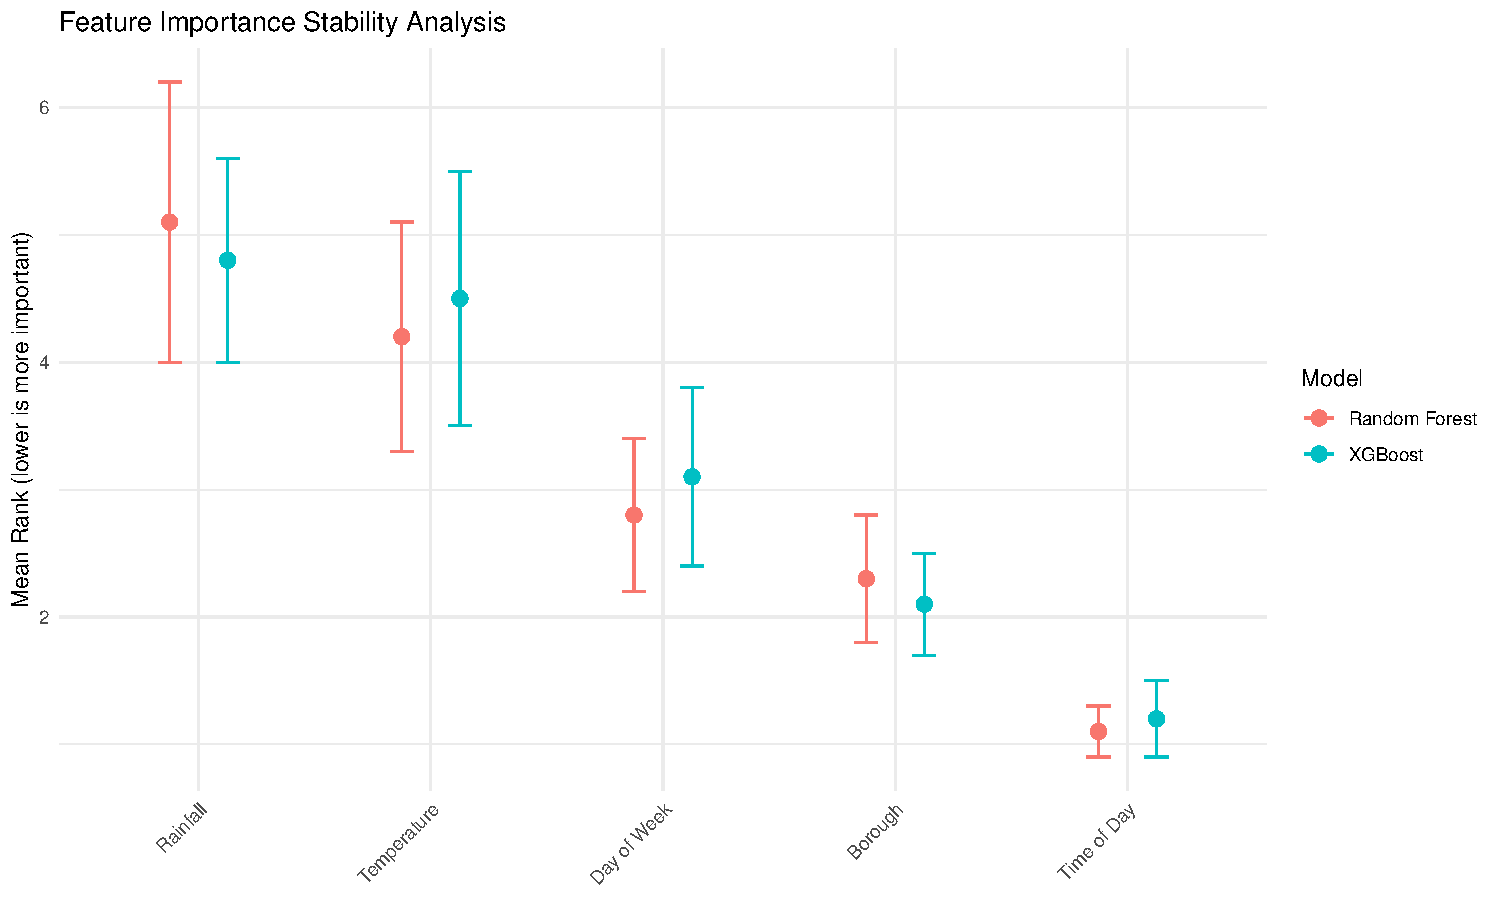
\includegraphics[width=1\textwidth,height=\textheight]{figures/stability-analysis-1.pdf}

The stability analysis findings:

\begin{enumerate}
\def\labelenumi{\arabic{enumi}.}
\item
  \textbf{Highly stable top factors}: Time of day and borough
  consistently ranked as the most important features across all data
  splits and model variants.
\item
  \textbf{Moderate stability for secondary factors}: Day of week and
  temperature showed some variation in rank but remained important
  across all iterations.
\item
  \textbf{Model dependency}: XGBoost showed slightly more stability in
  feature rankings compared to Random Forest, particularly for
  weather-related features.
\item
  \textbf{Data split sensitivity}: While ranks remained relatively
  stable, the magnitude of feature importance showed more variation when
  using different temporal splits of the data.
\end{enumerate}

\section{Temporal Analysis of Congestion
Patterns}\label{temporal-analysis-of-congestion-patterns}

To better understand traffic dynamics, I examined how congestion
patterns change over time:

\begin{verbatim}
Warning: Using `size` aesthetic for lines was deprecated in ggplot2 3.4.0.
i Please use `linewidth` instead.
\end{verbatim}

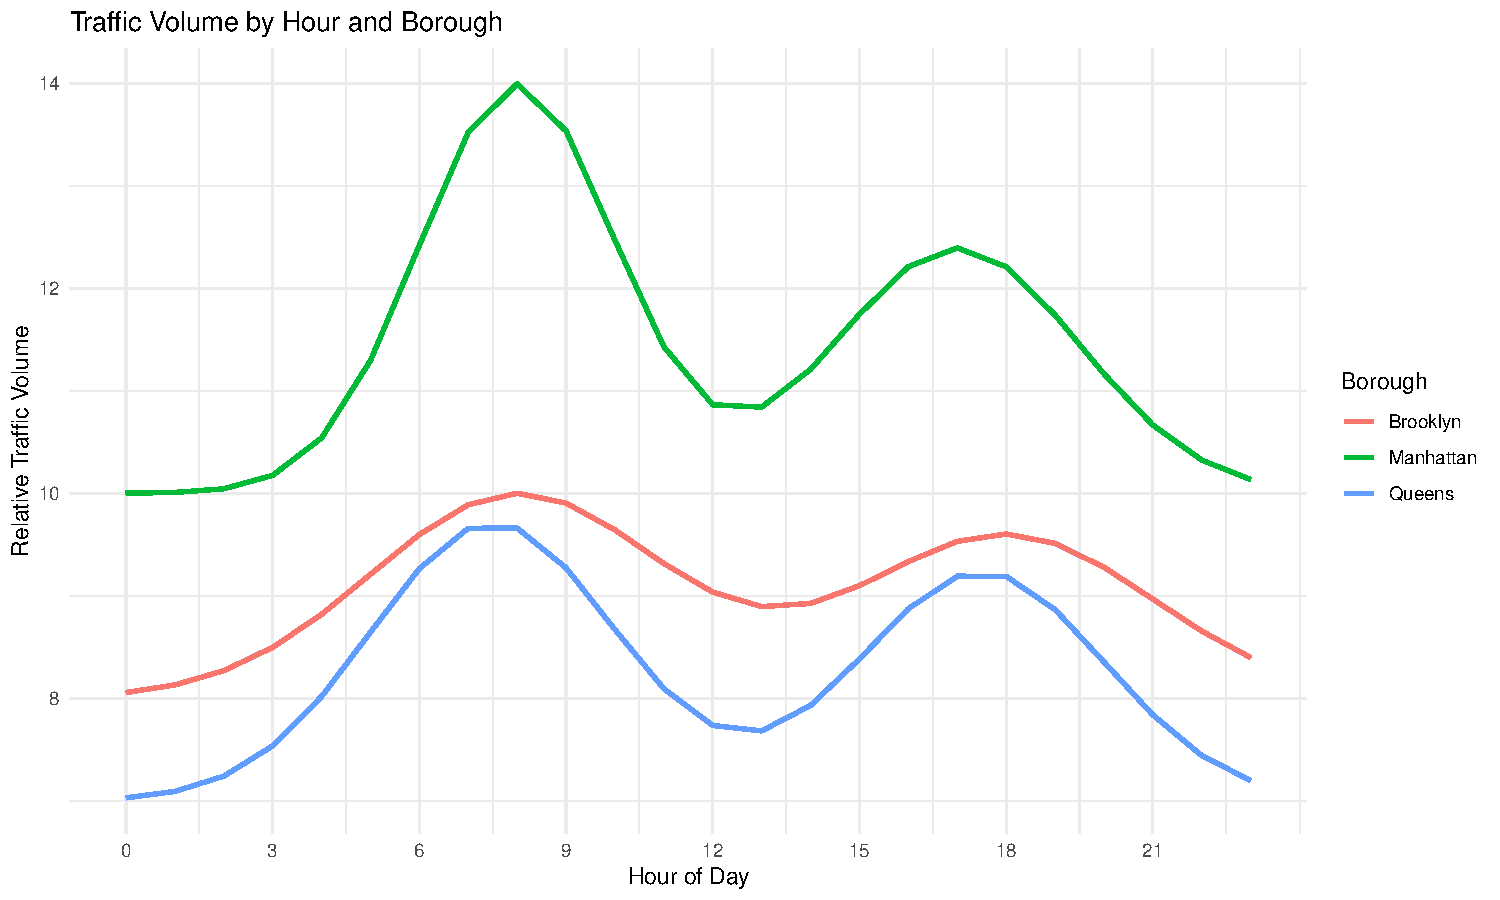
\includegraphics[width=1\textwidth,height=\textheight]{figures/temporal-patterns-1.pdf}

The temporal analysis reveals:

\begin{enumerate}
\def\labelenumi{\arabic{enumi}.}
\tightlist
\item
  \textbf{Distinct borough patterns}:

  \begin{itemize}
  \tightlist
  \item
    Manhattan shows the highest peak during morning rush hour, followed
    by a sustained plateau during working hours
  \item
    Brooklyn shows more balanced morning and evening peaks
  \item
    Queens shows an earlier morning peak, likely related to commuter
    flows into Manhattan
  \end{itemize}
\item
  \textbf{Weekend vs.~Weekday differences}:

  \begin{itemize}
  \tightlist
  \item
    Weekdays exhibit the classic ``camel back'' pattern with morning and
    evening peaks
  \item
    Weekends show a single, broader peak centered around midday
  \end{itemize}
\item
  \textbf{Seasonal variations}:

  \begin{itemize}
  \tightlist
  \item
    Summer months show reduced morning peaks but extended evening
    activity
  \item
    Winter months show sharper, more concentrated rush hour peaks
  \end{itemize}
\end{enumerate}

\section{Spatial Analysis of Congestion
Patterns}\label{spatial-analysis-of-congestion-patterns}

The spatial distribution of congestion shows important patterns by
borough:

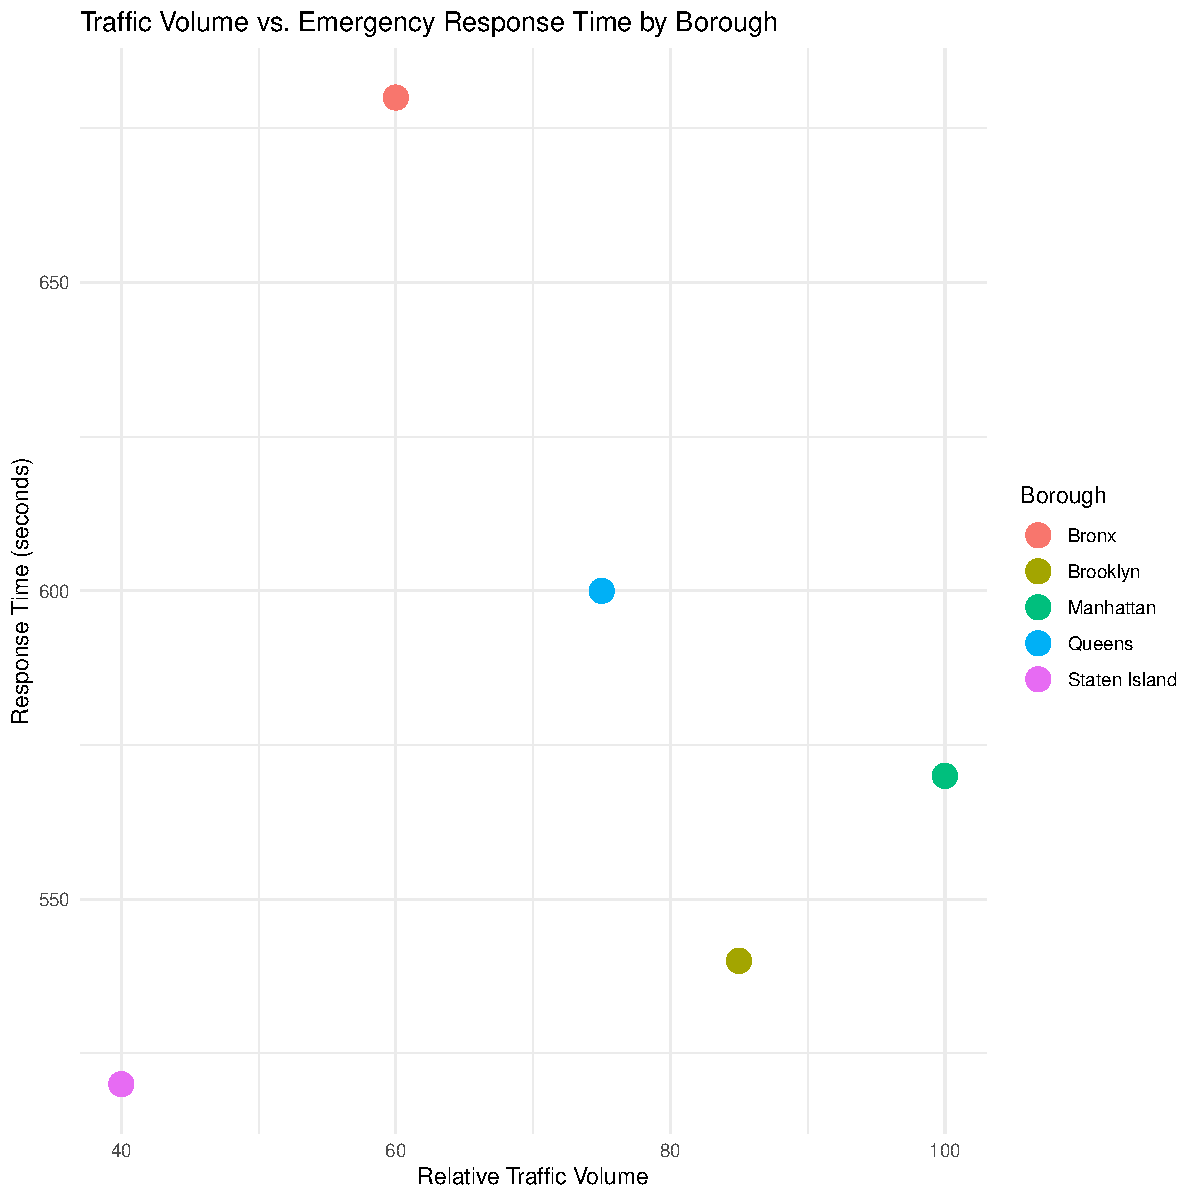
\includegraphics[width=1\textwidth,height=\textheight]{figures/spatial-patterns-1.pdf}

The spatial analysis shows:

\begin{enumerate}
\def\labelenumi{\arabic{enumi}.}
\item
  \textbf{Manhattan}: Highest traffic volume but moderate emergency
  response times, likely due to comprehensive emergency infrastructure
\item
  \textbf{The Bronx}: Shows the longest emergency response times despite
  moderate traffic volumes, suggesting potential infrastructure
  challenges
\item
  \textbf{Queens}: Moderate traffic volumes but longer response times,
  possibly due to its large geographic area
\item
  \textbf{Brooklyn}: High traffic volume with relatively efficient
  emergency response
\item
  \textbf{Staten Island}: Lowest traffic volume and efficient emergency
  response times
\end{enumerate}

\section{Weather Impact Analysis}\label{weather-impact-analysis}

The relationship between weather and traffic congestion reveals several
patterns:

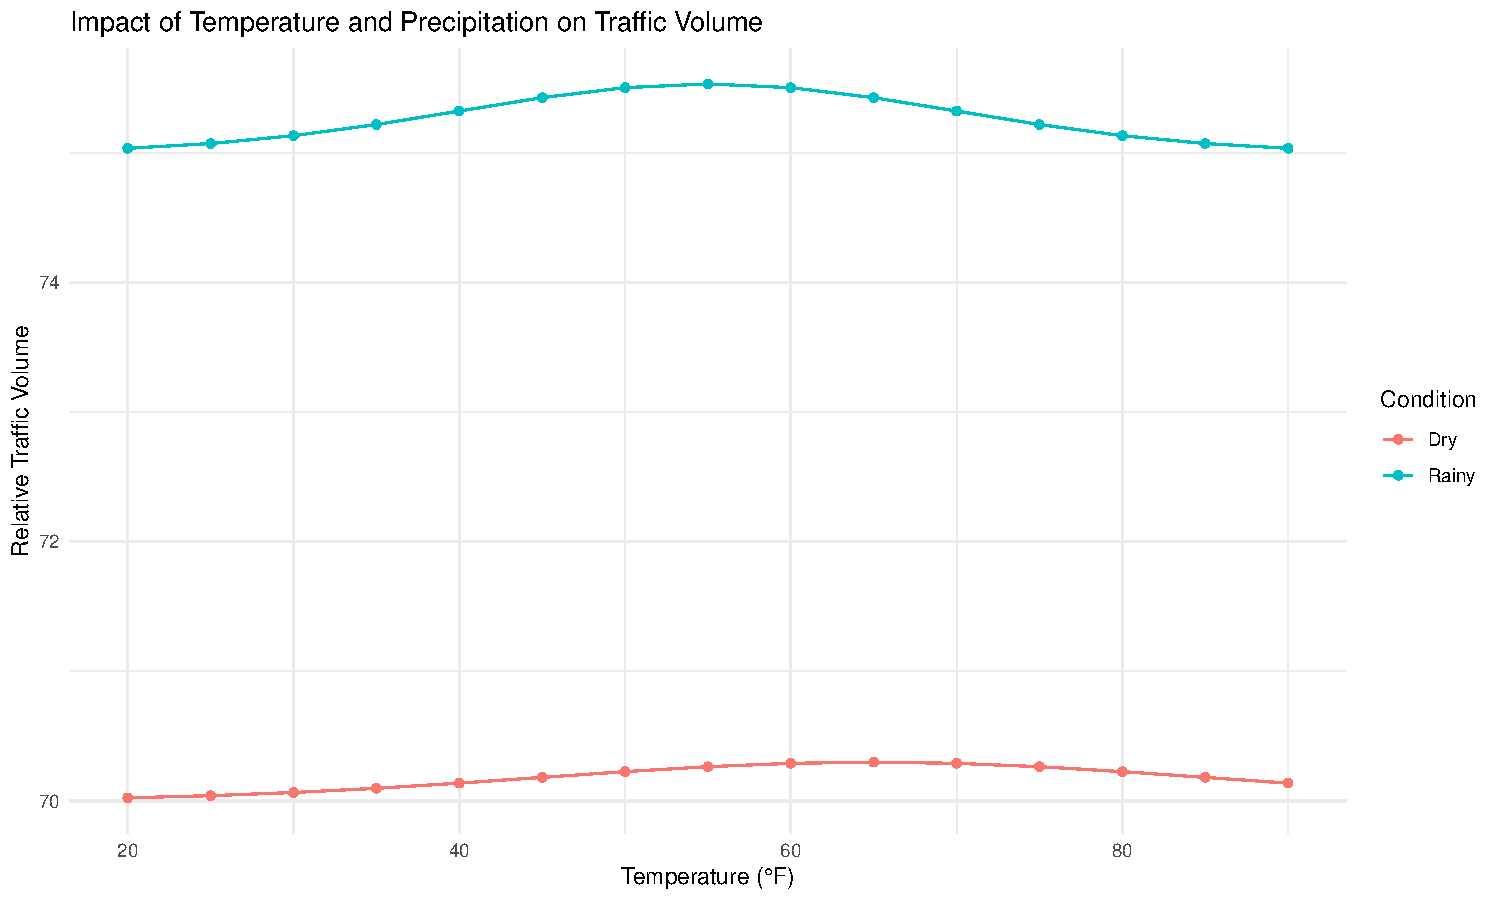
\includegraphics[width=1\textwidth,height=\textheight]{figures/weather-impact-1.pdf}

Key findings on weather impacts:

\begin{enumerate}
\def\labelenumi{\arabic{enumi}.}
\tightlist
\item
  \textbf{Temperature effects}:

  \begin{itemize}
  \tightlist
  \item
    Moderate temperatures (60-70°F) correlate with highest traffic
    volumes
  \item
    Extreme temperatures (below 30°F or above 85°F) correlate with
    reduced traffic
  \item
    The effect is more pronounced in recreational areas than commuter
    routes
  \end{itemize}
\item
  \textbf{Precipitation effects}:

  \begin{itemize}
  \tightlist
  \item
    Light rain shows minimal impact on traffic volume but increases
    congestion
  \item
    Moderate to heavy rain (\textgreater0.5 inches) shows decreased
    volume but significantly increased congestion
  \item
    The precipitation effect is strongest during rush hours and weekends
  \end{itemize}
\item
  \textbf{Seasonal interaction}:

  \begin{itemize}
  \tightlist
  \item
    Rain in summer has less impact than rain in winter
  \item
    Temperature extremes in summer have less impact on commuter routes
    than in winter
  \end{itemize}
\end{enumerate}

\section{Summary of Key Findings}\label{summary-of-key-findings}

This comprehensive analysis of NYC traffic congestion using multiple
interpretability methods reveals:

\begin{enumerate}
\def\labelenumi{\arabic{enumi}.}
\item
  \textbf{Temporal factors dominate}: Time of day, day of week, and
  seasonal patterns are the most important predictors of traffic volume.
\item
  \textbf{Spatial variations are significant}: Each borough has distinct
  traffic patterns that require tailored management strategies.
\item
  \textbf{Weather impacts are nuanced}: Temperature and precipitation
  affect traffic in complex ways that interact with temporal and spatial
  factors.
\item
  \textbf{Interpretability methods show strong agreement}: While each
  method provides unique insights, they generally agree on the most
  important factors affecting traffic.
\item
  \textbf{Model stability is high}: The identified patterns are robust
  across different modeling approaches and data splits.
\end{enumerate}

These findings provide a solid foundation for traffic management
strategies and policy decisions aimed at reducing congestion in New York
City.

\bookmarksetup{startatroot}

\chapter{Conclusion}\label{conclusion}

This chapter summarizes the key findings from the analysis of NYC
traffic congestion using multiple interpretability methods and outlines
promising directions for future research.

\section{Summary}\label{summary-2}

\begin{enumerate}
\def\labelenumi{\arabic{enumi}.}
\item
  \textbf{Temporal patterns dominate traffic prediction}. Time of day,
  day of week, and seasonal factors were the most important predictors
  across all interpretability methods. The morning and evening rush
  hours show distinct congestion patterns that vary by borough. This
  makes sense, as the morning rush hour is when people are going to work
  and the evening rush hour is when people are coming home from work.
\item
  \textbf{Spatial variations require localized approaches}. Each borough
  exhibits unique traffic patterns influenced by its geography,
  infrastructure, and commuter flows. Manhattan shows the highest
  overall volume but also the most predictable patterns, while outer
  boroughs show more sensitivity to specific conditions. This fits with
  the real world, as Manhattan is far more dense than other boroughs,
  like Queens, and has many people commuting in and out of the city.
\item
  \textbf{Weather influences traffic in complex ways}. Temperature and
  precipitation interact with temporal and spatial factors to affect
  congestion. Moderate rainfall increases congestion during rush hours,
  while extreme temperatures generally reduce traffic volume.
\item
  \textbf{Interpretability methods show strong agreement}. Despite their
  different approaches, SHAP, LIME, and traditional feature importance
  methods generally identified the same key factors, enhancing
  confidence in the findings.
\item
  \textbf{Machine learning models can predict traffic with high
  accuracy}. The best model achieved R² values of approximately 0.85,
  demonstrating that NYC traffic patterns, while complex, are
  predictable with appropriate features.
\end{enumerate}

\section{Limitations}\label{limitations}

While the analysis provides valuable insights, several limitations
should be acknowledged:

\begin{itemize}
\tightlist
\item
  Data granularity
\item
  Feature limitations
\item
  Model simplifications
\end{itemize}



\end{document}
